%%%%%%%%%%%%%%%%%%%%%%%%%%%%%%%%%%%%%%%%%%%%%%%%%%%%%%%%%%%%%%%

% Set up document

\documentclass{beamer}
\usecolortheme{whale}
\setbeamersize{text margin left=5mm,text margin right=5mm}

% Used to create a section slide between section
\AtBeginSection[]{
  \begin{frame}
  \vfill
  \centering
  \begin{beamercolorbox}[sep=8pt,center,shadow=true,rounded=true]{title}
    \usebeamerfont{title}\insertsectionhead\par%
  \end{beamercolorbox}
  \vfill
  \end{frame}
}

% Remove default navigation symbols and add just  page number
\setbeamertemplate{navigation symbols}{} % Clear default navigation
\addtobeamertemplate{navigation symbols}{}{%
    \usebeamerfont{footline}%
    \usebeamercolor[fg]{footline}%
    \hspace{1em}%
    \insertframenumber/\inserttotalframenumber
}


%%%%%%%%%%%%%%%%%%%%%%%%%%%%%%%%%%%%%%%%%%%%%%%%%%%%%%%%%%%%%%%

% Title page

\title{Stroke Audit Machine Learning (SAMueL)}
\subtitle{Learnings from explainable machine learning}


\author{Kerry Pearn\inst{1}, Michael Allen\inst{1,3}, Anna Laws\inst{1}, Richard Everson\inst{3}, Martin James\inst{1,2} }
\institute{\inst{1}University of Exeter Medical School \inst{2}Royal Devon University Healthcare NHS Foundation Trust \inst{3}University of Exeter Institute of Data Science and Artificial Intelligence}

%\institute{Overleaf}
\date{January 2023}


\begin{document}

%\frame{\titlepage}

\begin{frame}
\titlepage


\end{frame}

%%%%%%%%%%%%%%%%%%%%%%%%%%%%%%%%%%%%%%%%%%%%%%%%%%%%%%%%%%%%%%%

\begin{frame}
\frametitle{Thrombolysis rates vary .... a lot}
Here we show the range of thrombolysis use across the 132 acute stroke centres in England and Wales.
\begin{center}
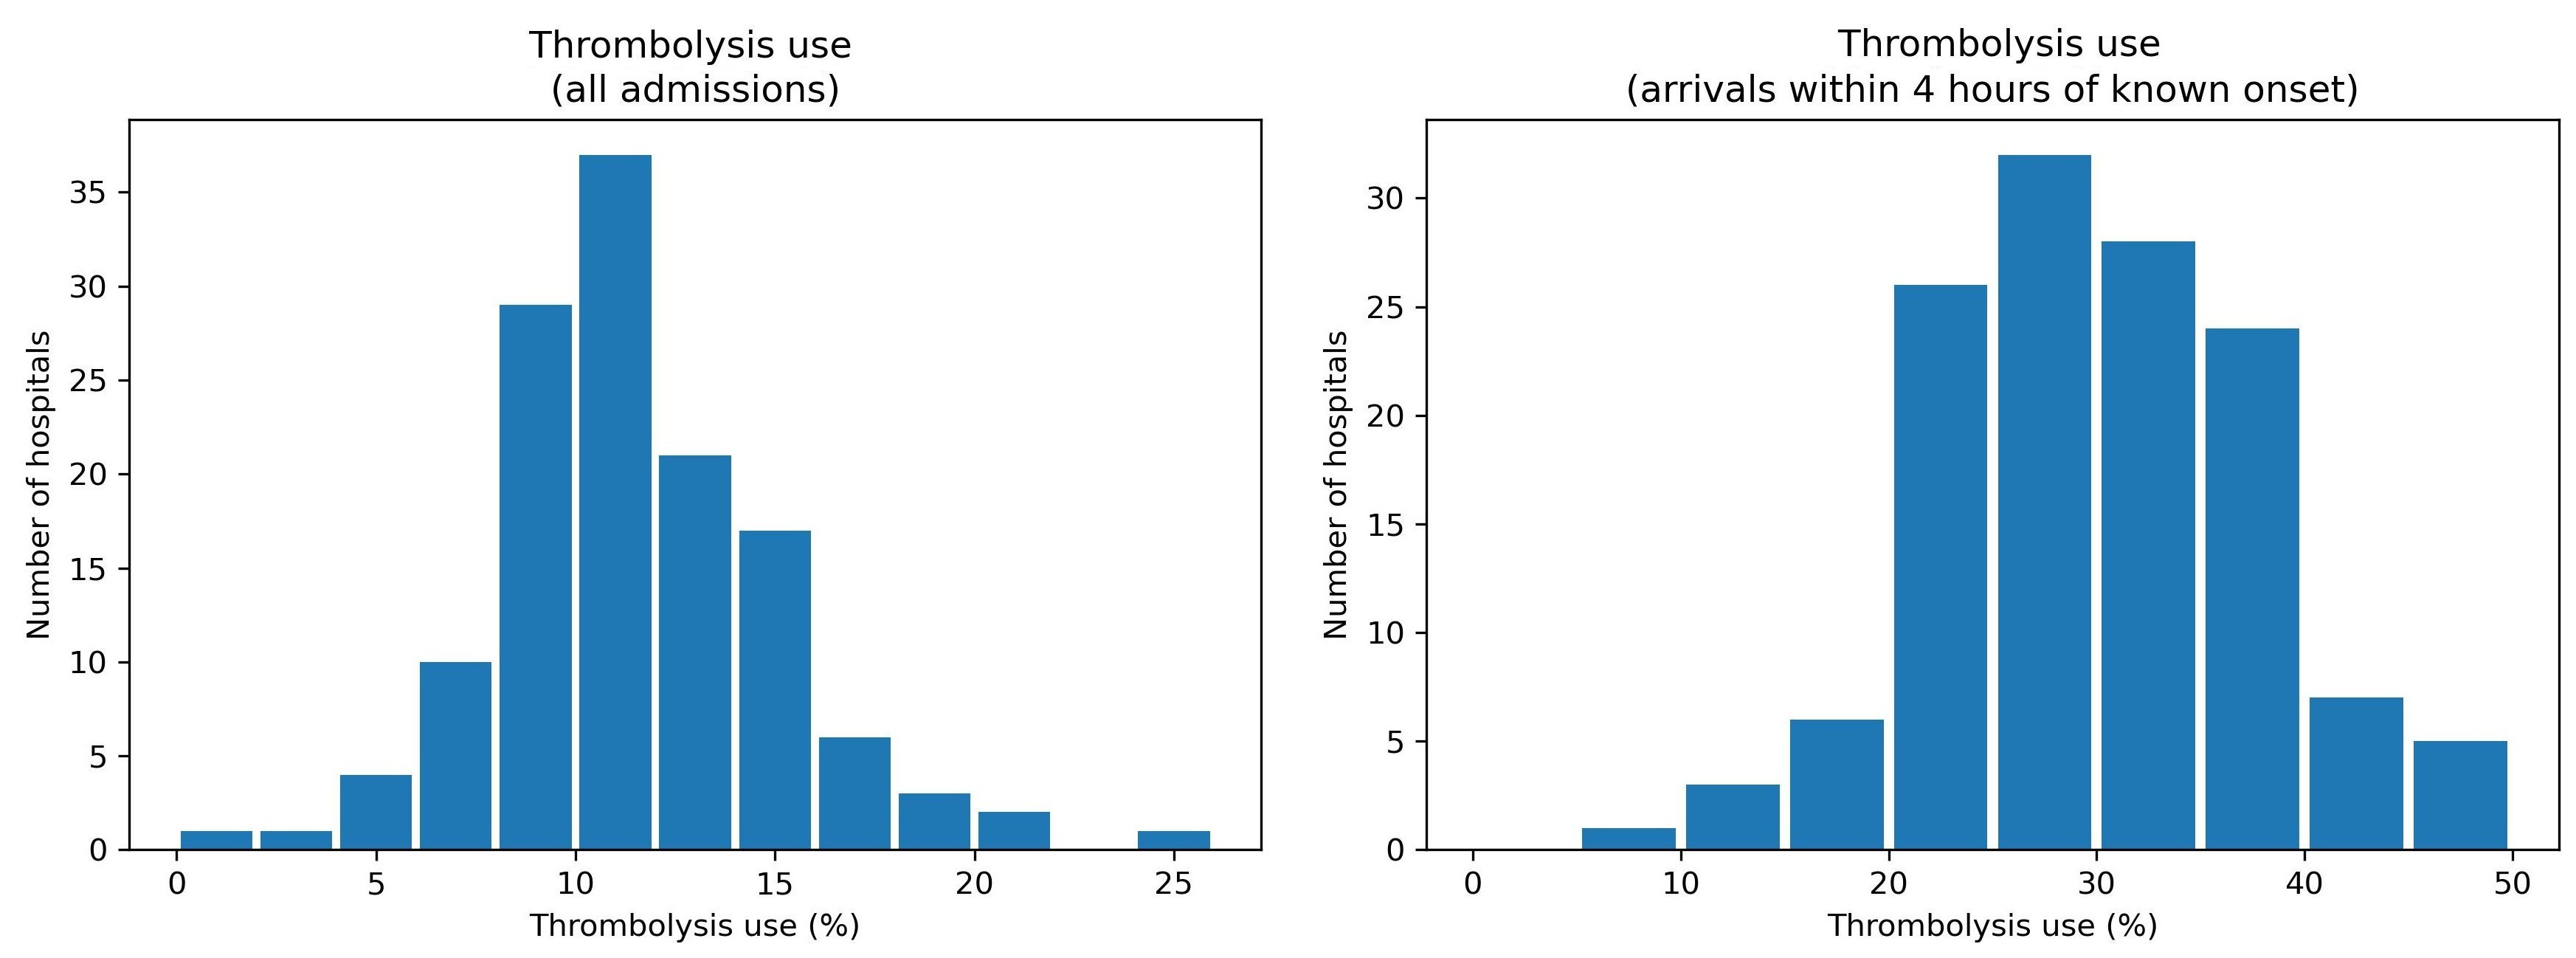
\includegraphics[width=1.0\textwidth]{./images/thrombolysis_hist}
\end{center}

How much of this variation is due to differences in decisions hospitals make on who they would give thrombolysis to?
\end{frame}

%%%%%%%%%%%%%%%%%%%%%%%%%%%%%%%%%%%%%%%%%%%%%%%%%%%%%%%%%%%%%%%

\begin{frame}
\frametitle{Our Approach}

\small

\begin{itemize}
    \item Train a machine learning algorithm to learn to predict to which patients each hospital would, or would not, give thrombolysis.
    \item Identify the patient characteristics which are most important in predicting use of thrombolysis, and produce a simpler machine learning model based on these characteristics.
    \item Identify \emph{ideal} candidates for thrombolysis.
    \item Add an \emph{explainable machine learning} layer* to understand patterns of use of thrombolysis.
    \item Investigate what we think would happen if every hospital received exactly the same 10k cohort of patients.
    \item Identify key subgroups of patients where hospitals differ in their use of thrombolysis.
\end{itemize}

\vspace{3mm}
\footnotesize
*SHAP (Shapley Additive Values, which provide information on what contribution each patient characteristic makes to the final prediction of whether they will, or will not, receive thrombolysis).
\end{frame}



%%%%%%%%%%%%%%%%%%%%%%%%%%%%%%%%%%%%%%%%%%%%%%%%%%%%%%%%%%%%%%%

\begin{frame}
\frametitle{Machine learning overview}
\begin{center}
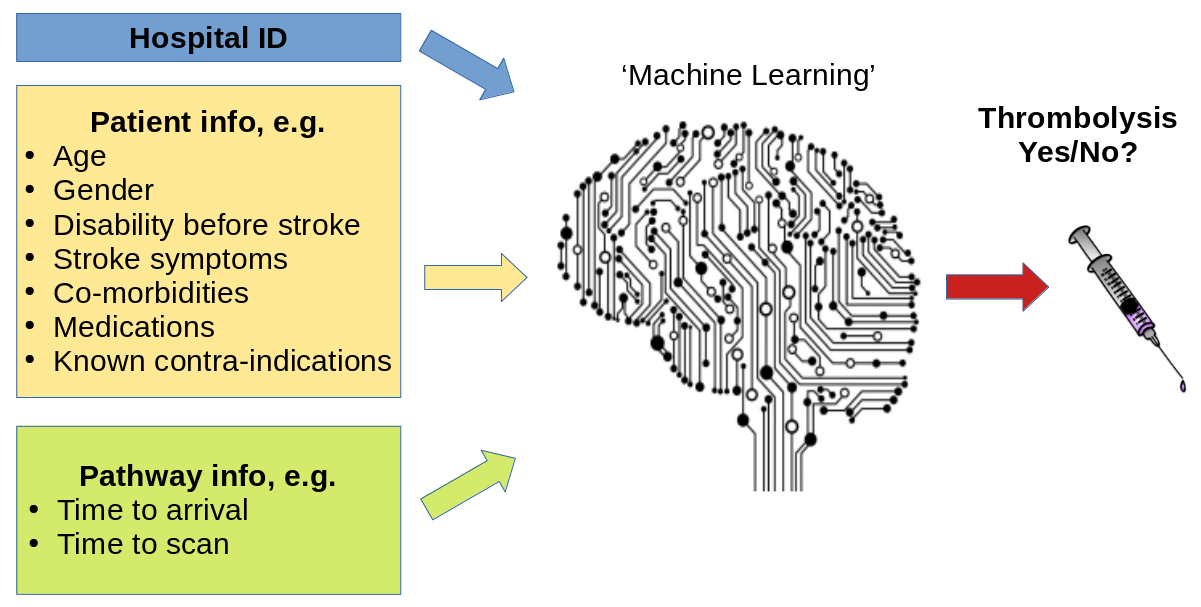
\includegraphics[width=0.80\textwidth]{./images/ml_model_high_level}
\end{center}

\small
Machine learning is based on the simple principle of recognising similarity to what has been seen before.
\vspace{3mm}

We accessed 246,676 emergency stroke admissions in England and Wales over three years. Our machine learning models use XGBoost classification, and are based on those 88,928 patients who arrive within 4 hours of known stroke onset. 
\end{frame}

%%%%%%%%%%%%%%%%%%%%%%%%%%%%%%%%%%%%%%%%%%%%%%%%%%%%%%%%%%%%%%%

\begin{frame}{Model accuracy, and simplification}

A model with all available 84 features had an ROC AUC of 0.922. A model with 10 features had an ROC AUC of 0.919.

\begin{center}
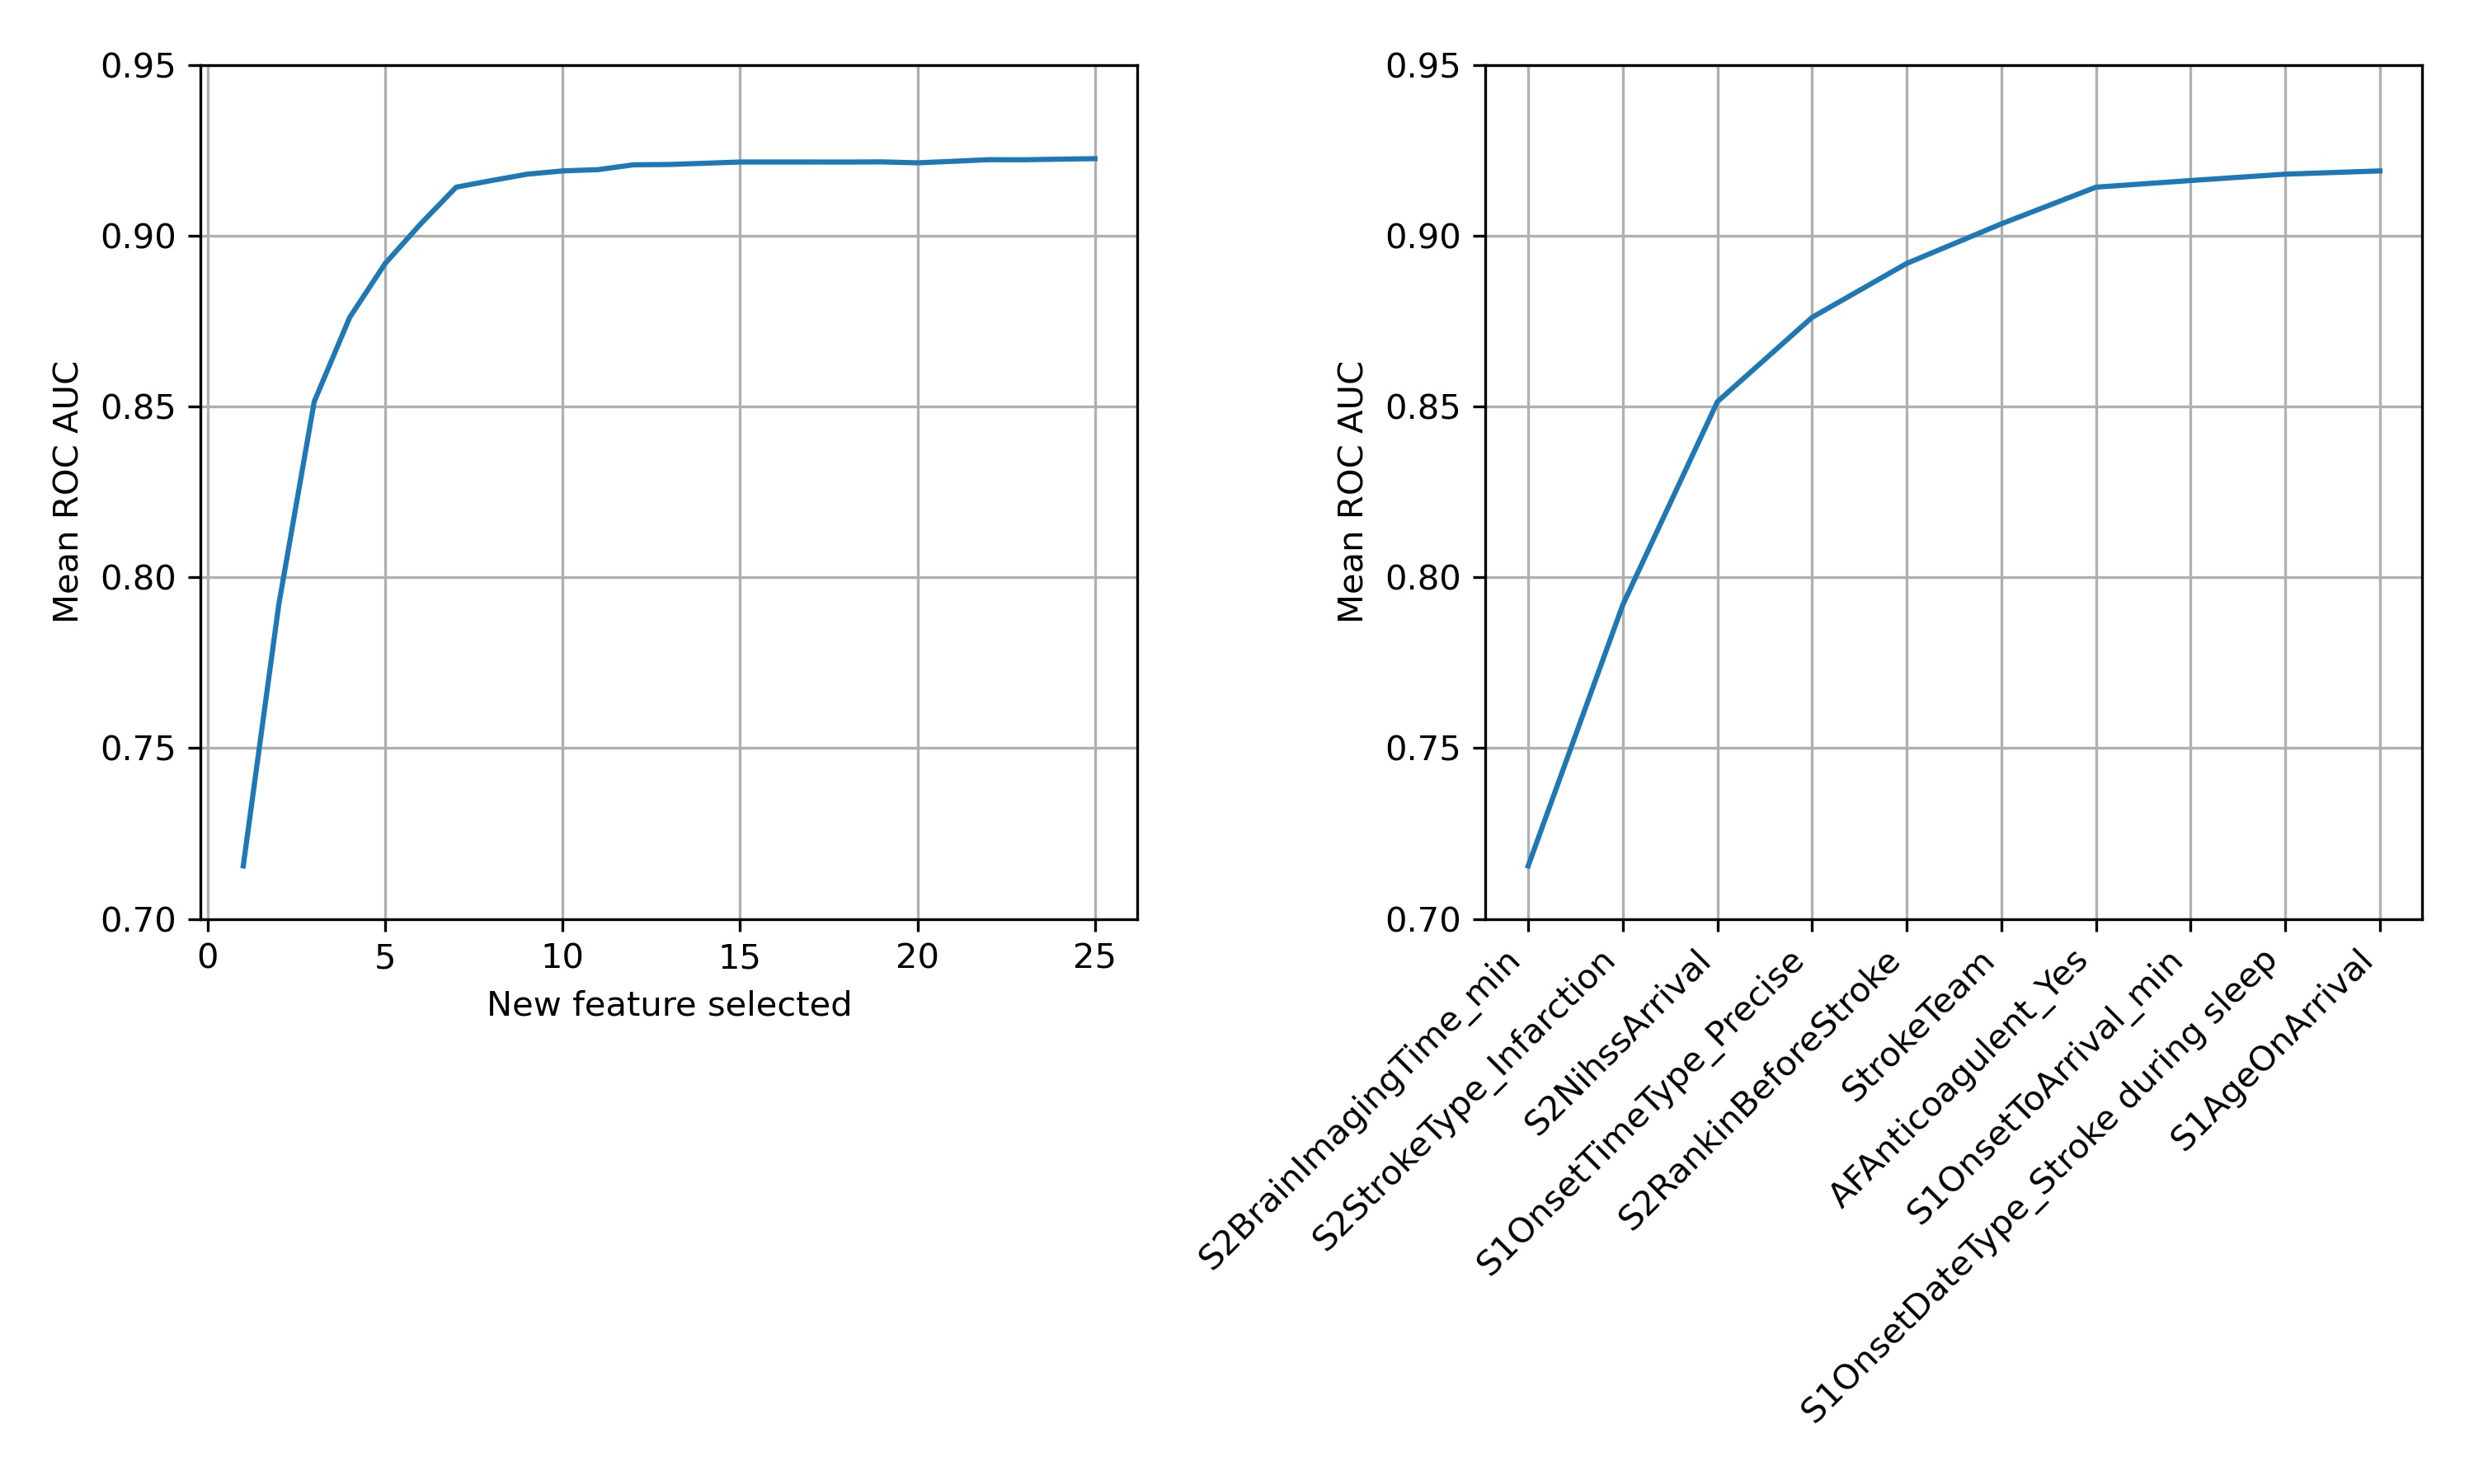
\includegraphics[width=0.9\textwidth]{./images/01_feature_selection.jpg}
\end{center}

Our simpler machine learning model will just use these 10 features.

\end{frame}


%%%%%%%%%%%%%%%%%%%%%%%%%%%%%%%%%%%%%%%%%%%%%%%%%%%%%%%%%%%%%%%

\begin{frame}{What do the most thrombolysable patients look like?}

\scriptsize For each hospital we identify the patient with the highest probability of receiving thrombolysis. Here we compare the range of feature values for these 'Most thrombolysable' patients with 1) All patients, 2) Thrombolysed patients, and 3) Non-thrombolysed patients.


\begin{center}
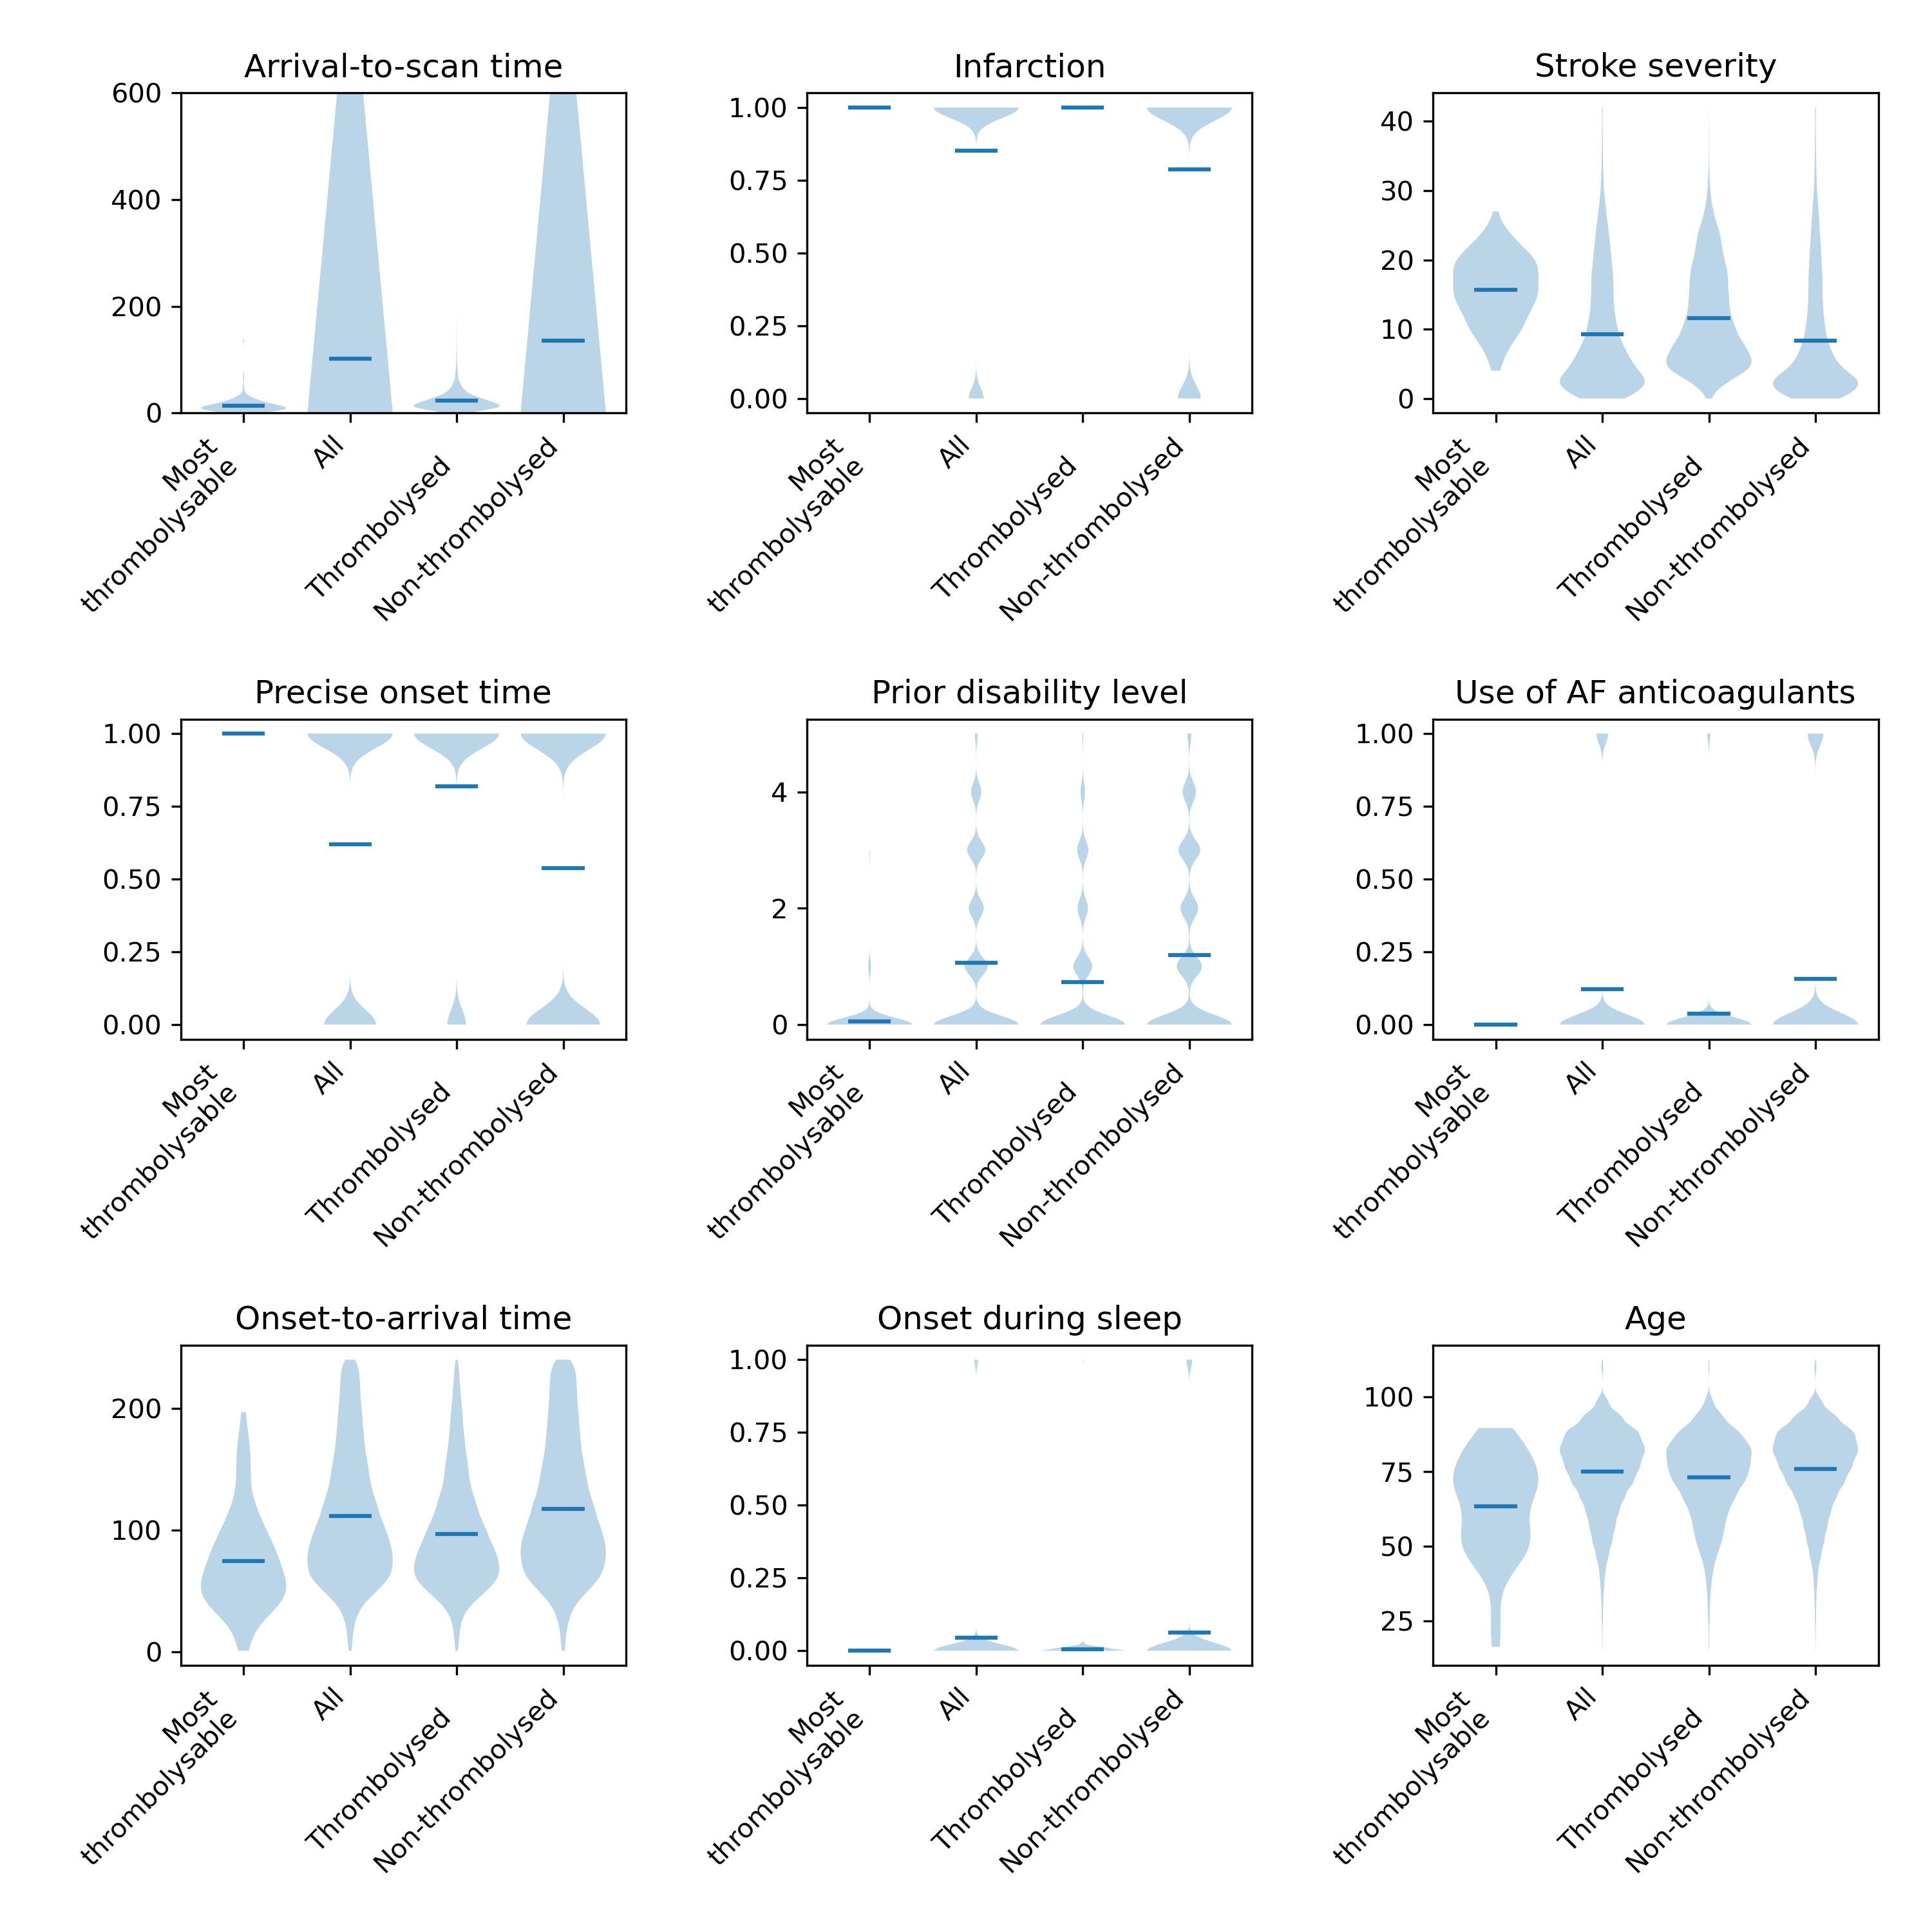
\includegraphics[width=0.63\textwidth]{./images/02a_most_thrombolsyable_violin.jpg}
\end{center}

\end{frame}

%%%%%%%%%%%%%%%%%%%%%%%%%%%%%%%%%%%%%%%%%%%%%%%%%%%%%%%%%%%%%%%

\begin{frame}{What do the most thrombolysable patients look like?}

Compared with other patients, the  most thrombolysable patients:

\vspace{3mm}

\begin{itemize}
\item Had shorter arrrival-to-scan times
\item Had an infarction stroke type
\item Had stroke severities with NIHR 5-25
\item Had a precise onset time
\item Had lower pre-stroke disability
\item Were not taking anticoagulant medication
\item Had shorter onset-to-arrival times
\item Did not have onset during sleep
\item Were younger
\end{itemize}

\vspace{3mm}

But, can we learn to be more \emph{quantitative} than this?

\end{frame}





%%%%%%%%%%%%%%%%%%%%%%%%%%%%%%%%%%%%%%%%%%%%%%%%%%%%%%%%%%%%%%%

\begin{frame}
\frametitle{Explaining model predictions with SHAP values}

SHAP values show the influence of features (even for \emph{`black box'} models).

\begin{center}
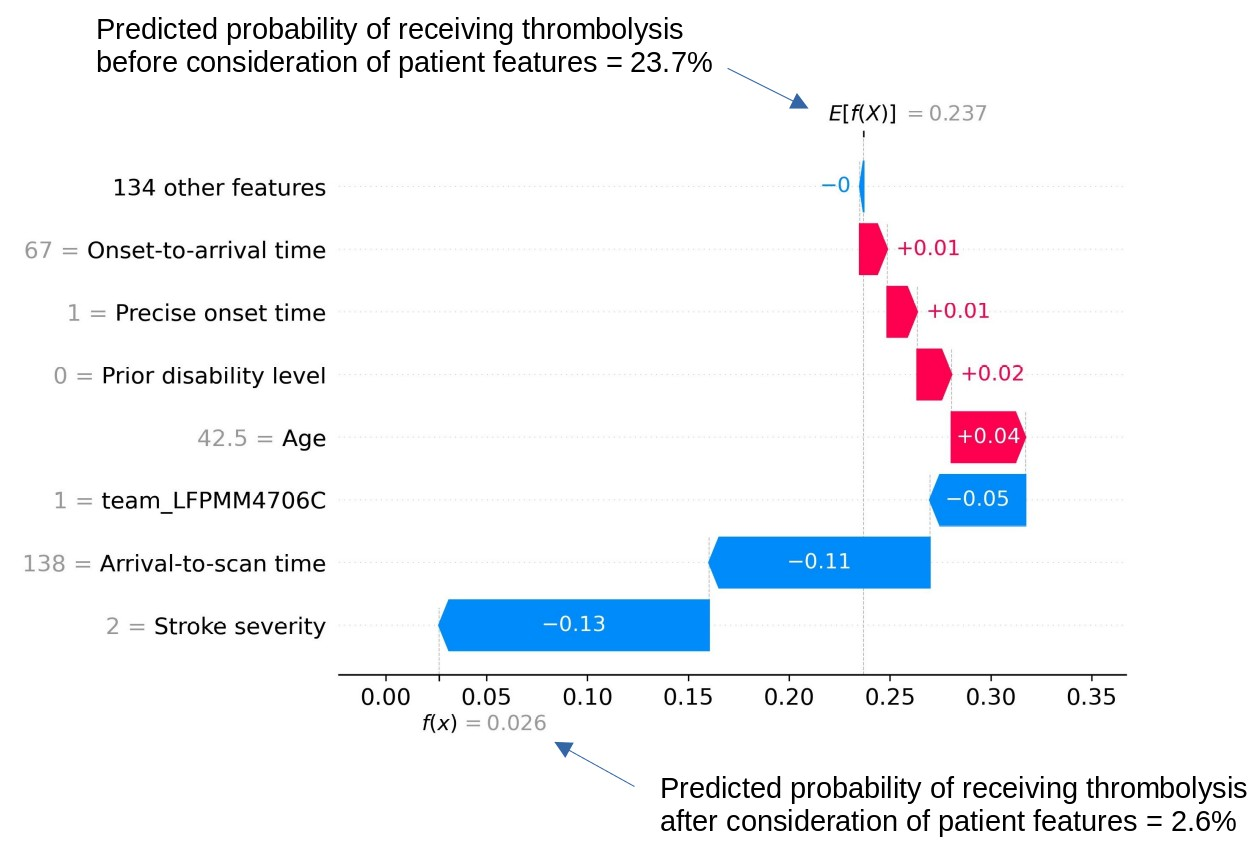
\includegraphics[width=0.90\textwidth]{./images/waterfall.jpg}
\end{center}
\end{frame}


%%%%%%%%%%%%%%%%%%%%%%%%%%%%%%%%%%%%%%%%%%%%%%%%%%%%%%%%%%%%%%%

\begin{frame}
\frametitle{What drives use of thrombolysis across all hospitals?}

\footnotesize{Note: SHAP values here are \emph{log odds}. Each step-change in value of \textpm 1 changes the chances of receiving thrombolysis about 3-fold. (Plots are in order of feature importance.)}

\begin{center}
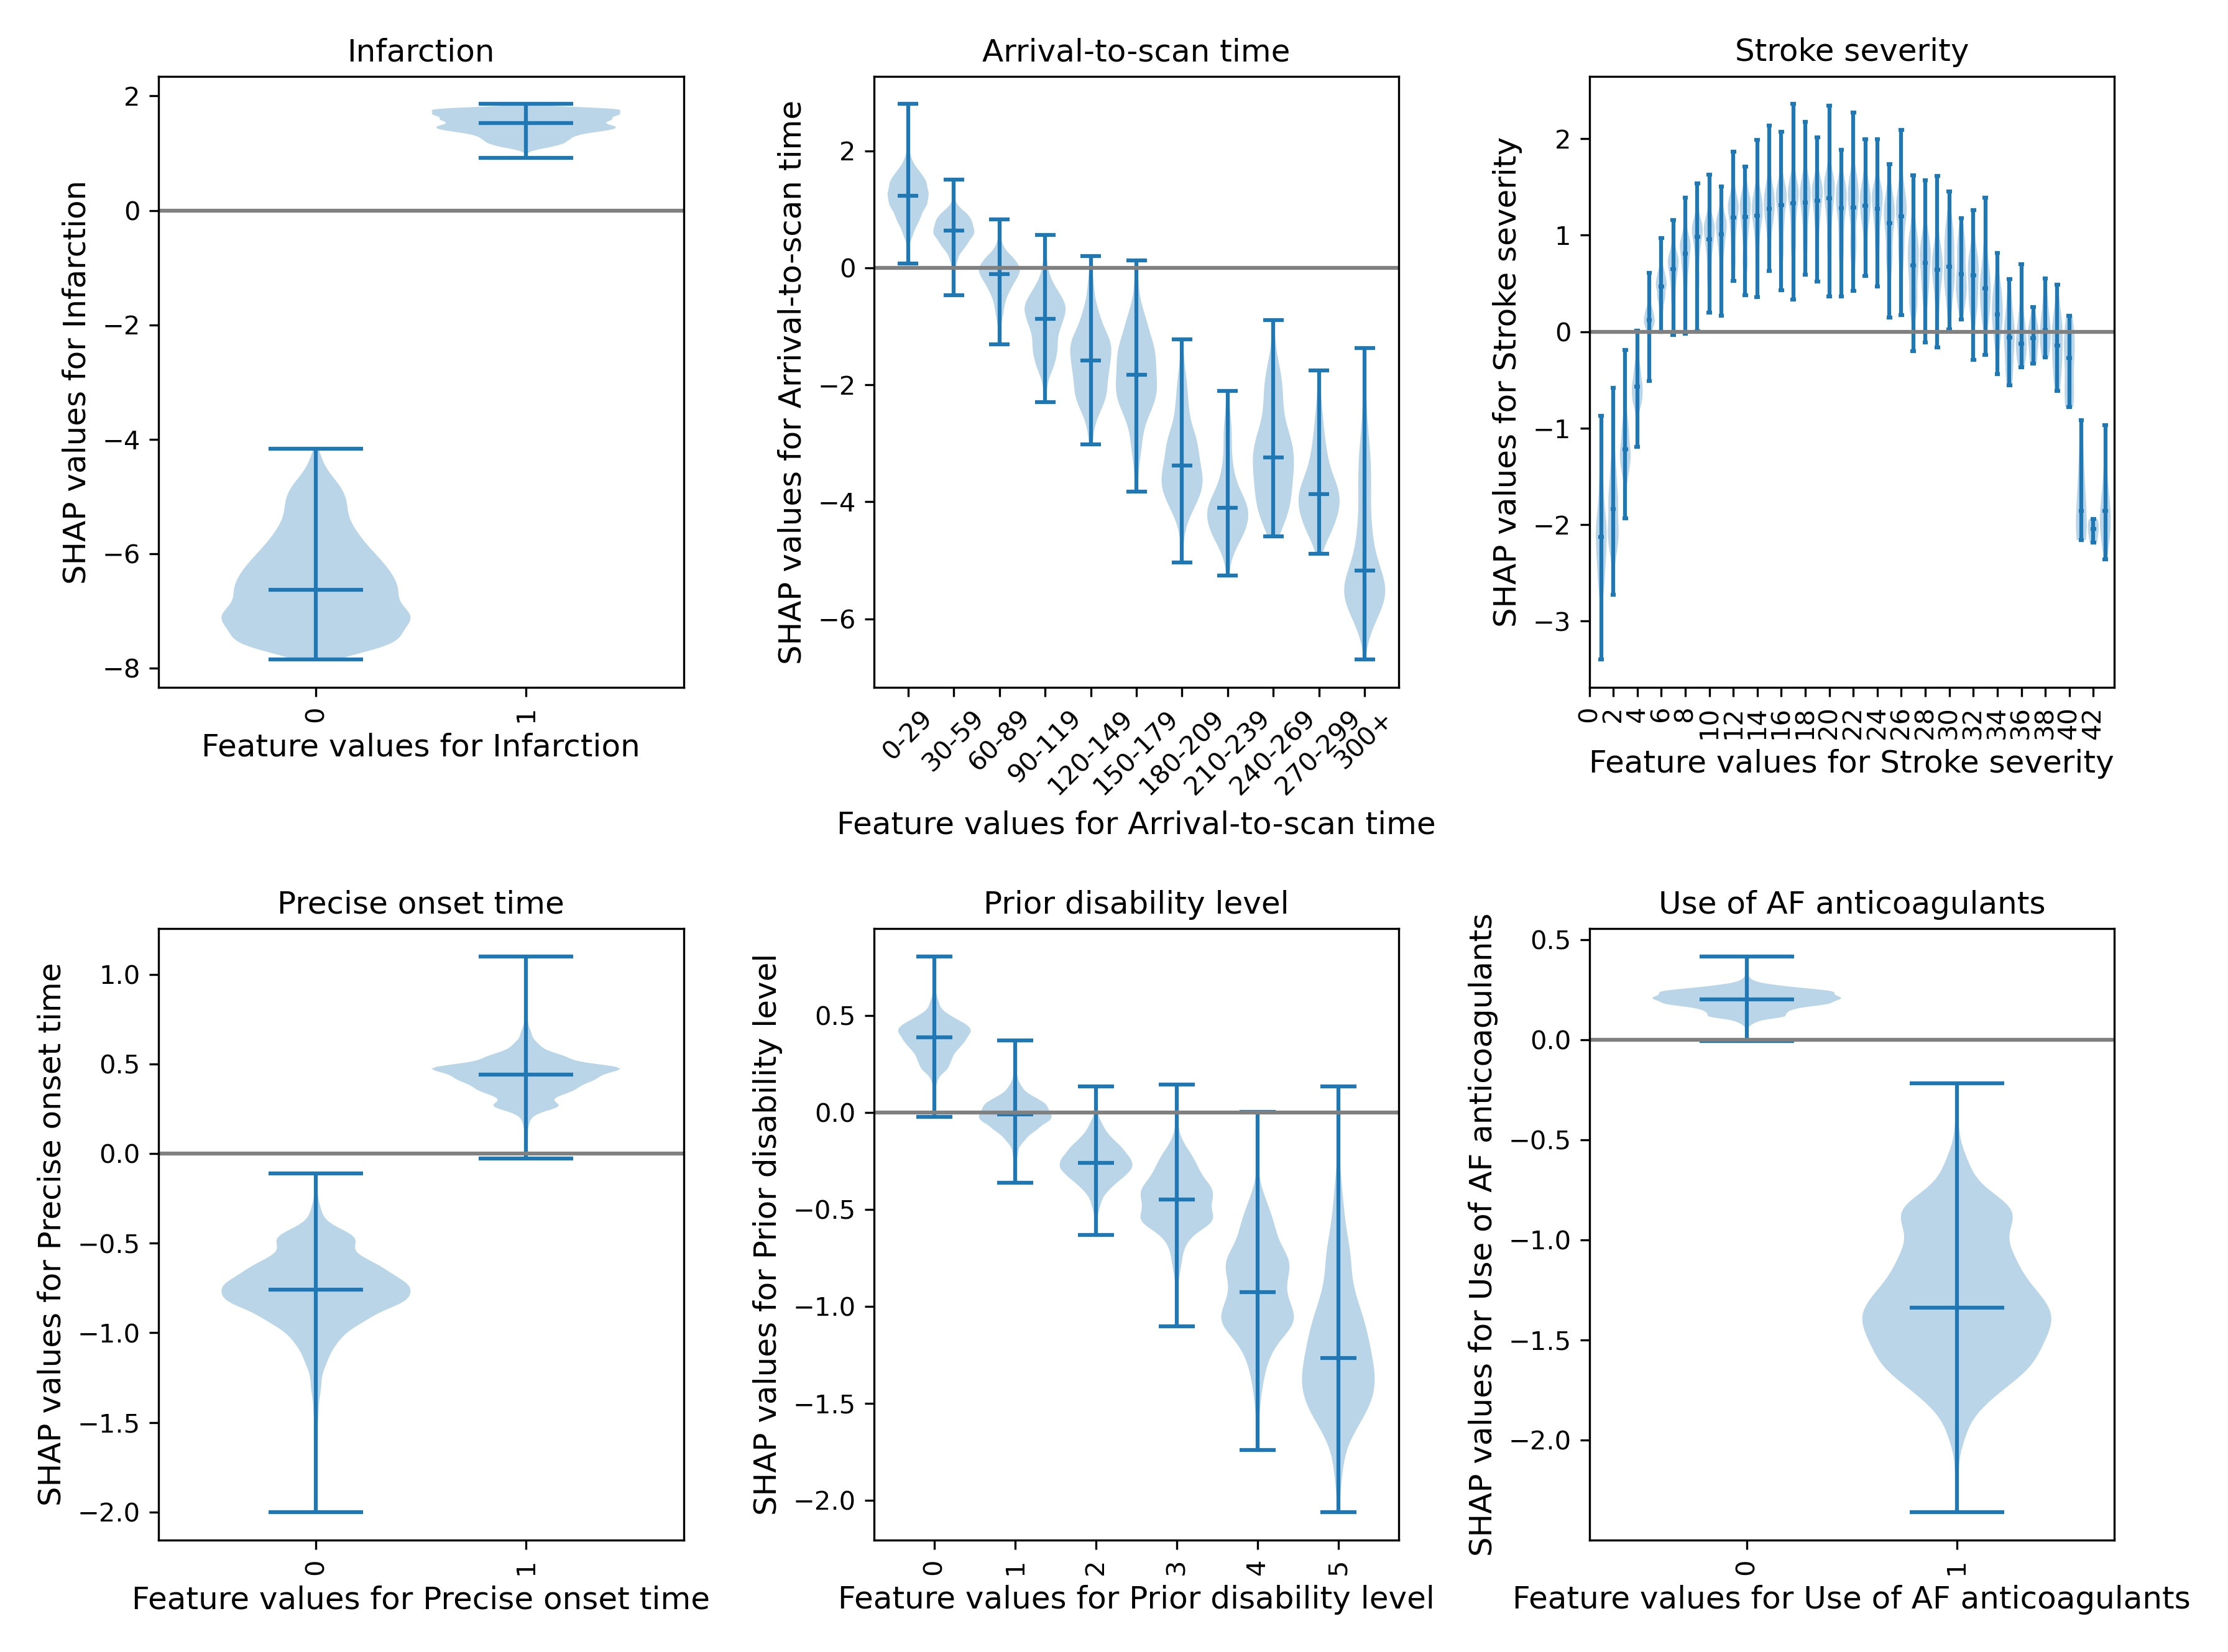
\includegraphics[width=0.80\textwidth]{./images/03_xgb_10_features_thrombolysis_shap_violin.jpg}
\end{center}
\end{frame}

%%%%%%%%%%%%%%%%%%%%%%%%%%%%%%%%%%%%%%%%%%%%%%%%%%%%%%%%%%%%%%%

\begin{frame}
\frametitle{What drives use of thrombolysis across all hospitals?}

The XGBoost/SHAP model revealed that the odds of receiving thrombolysis:

\begin{itemize}
    \item Reduced 20 fold over the first 100 minutes of arrival-to-scan time.
    \item Varied 30 fold depending on stroke severity.
    \item Reduced 3 fold with imprecise onset time.
    \item Fell 5 fold with increasing pre-stroke disability.
    \item Varied 15 fold between hospitals. 
\end{itemize}

\end{frame}

%%%%%%%%%%%%%%%%%%%%%%%%%%%%%%%%%%%%%%%%%%%%%%%%%%%%%%%%%%%%%%%

\begin{frame}
\frametitle{Hospital SHAP predicts a hospital's predisposition to use thrombolysis}

\footnotesize Here we show the relationship of hospital SHAP with the hospital thrombolysis use for 1) the hospitals own patients, and 2) a common 10k cohort of patients.

\begin{center}
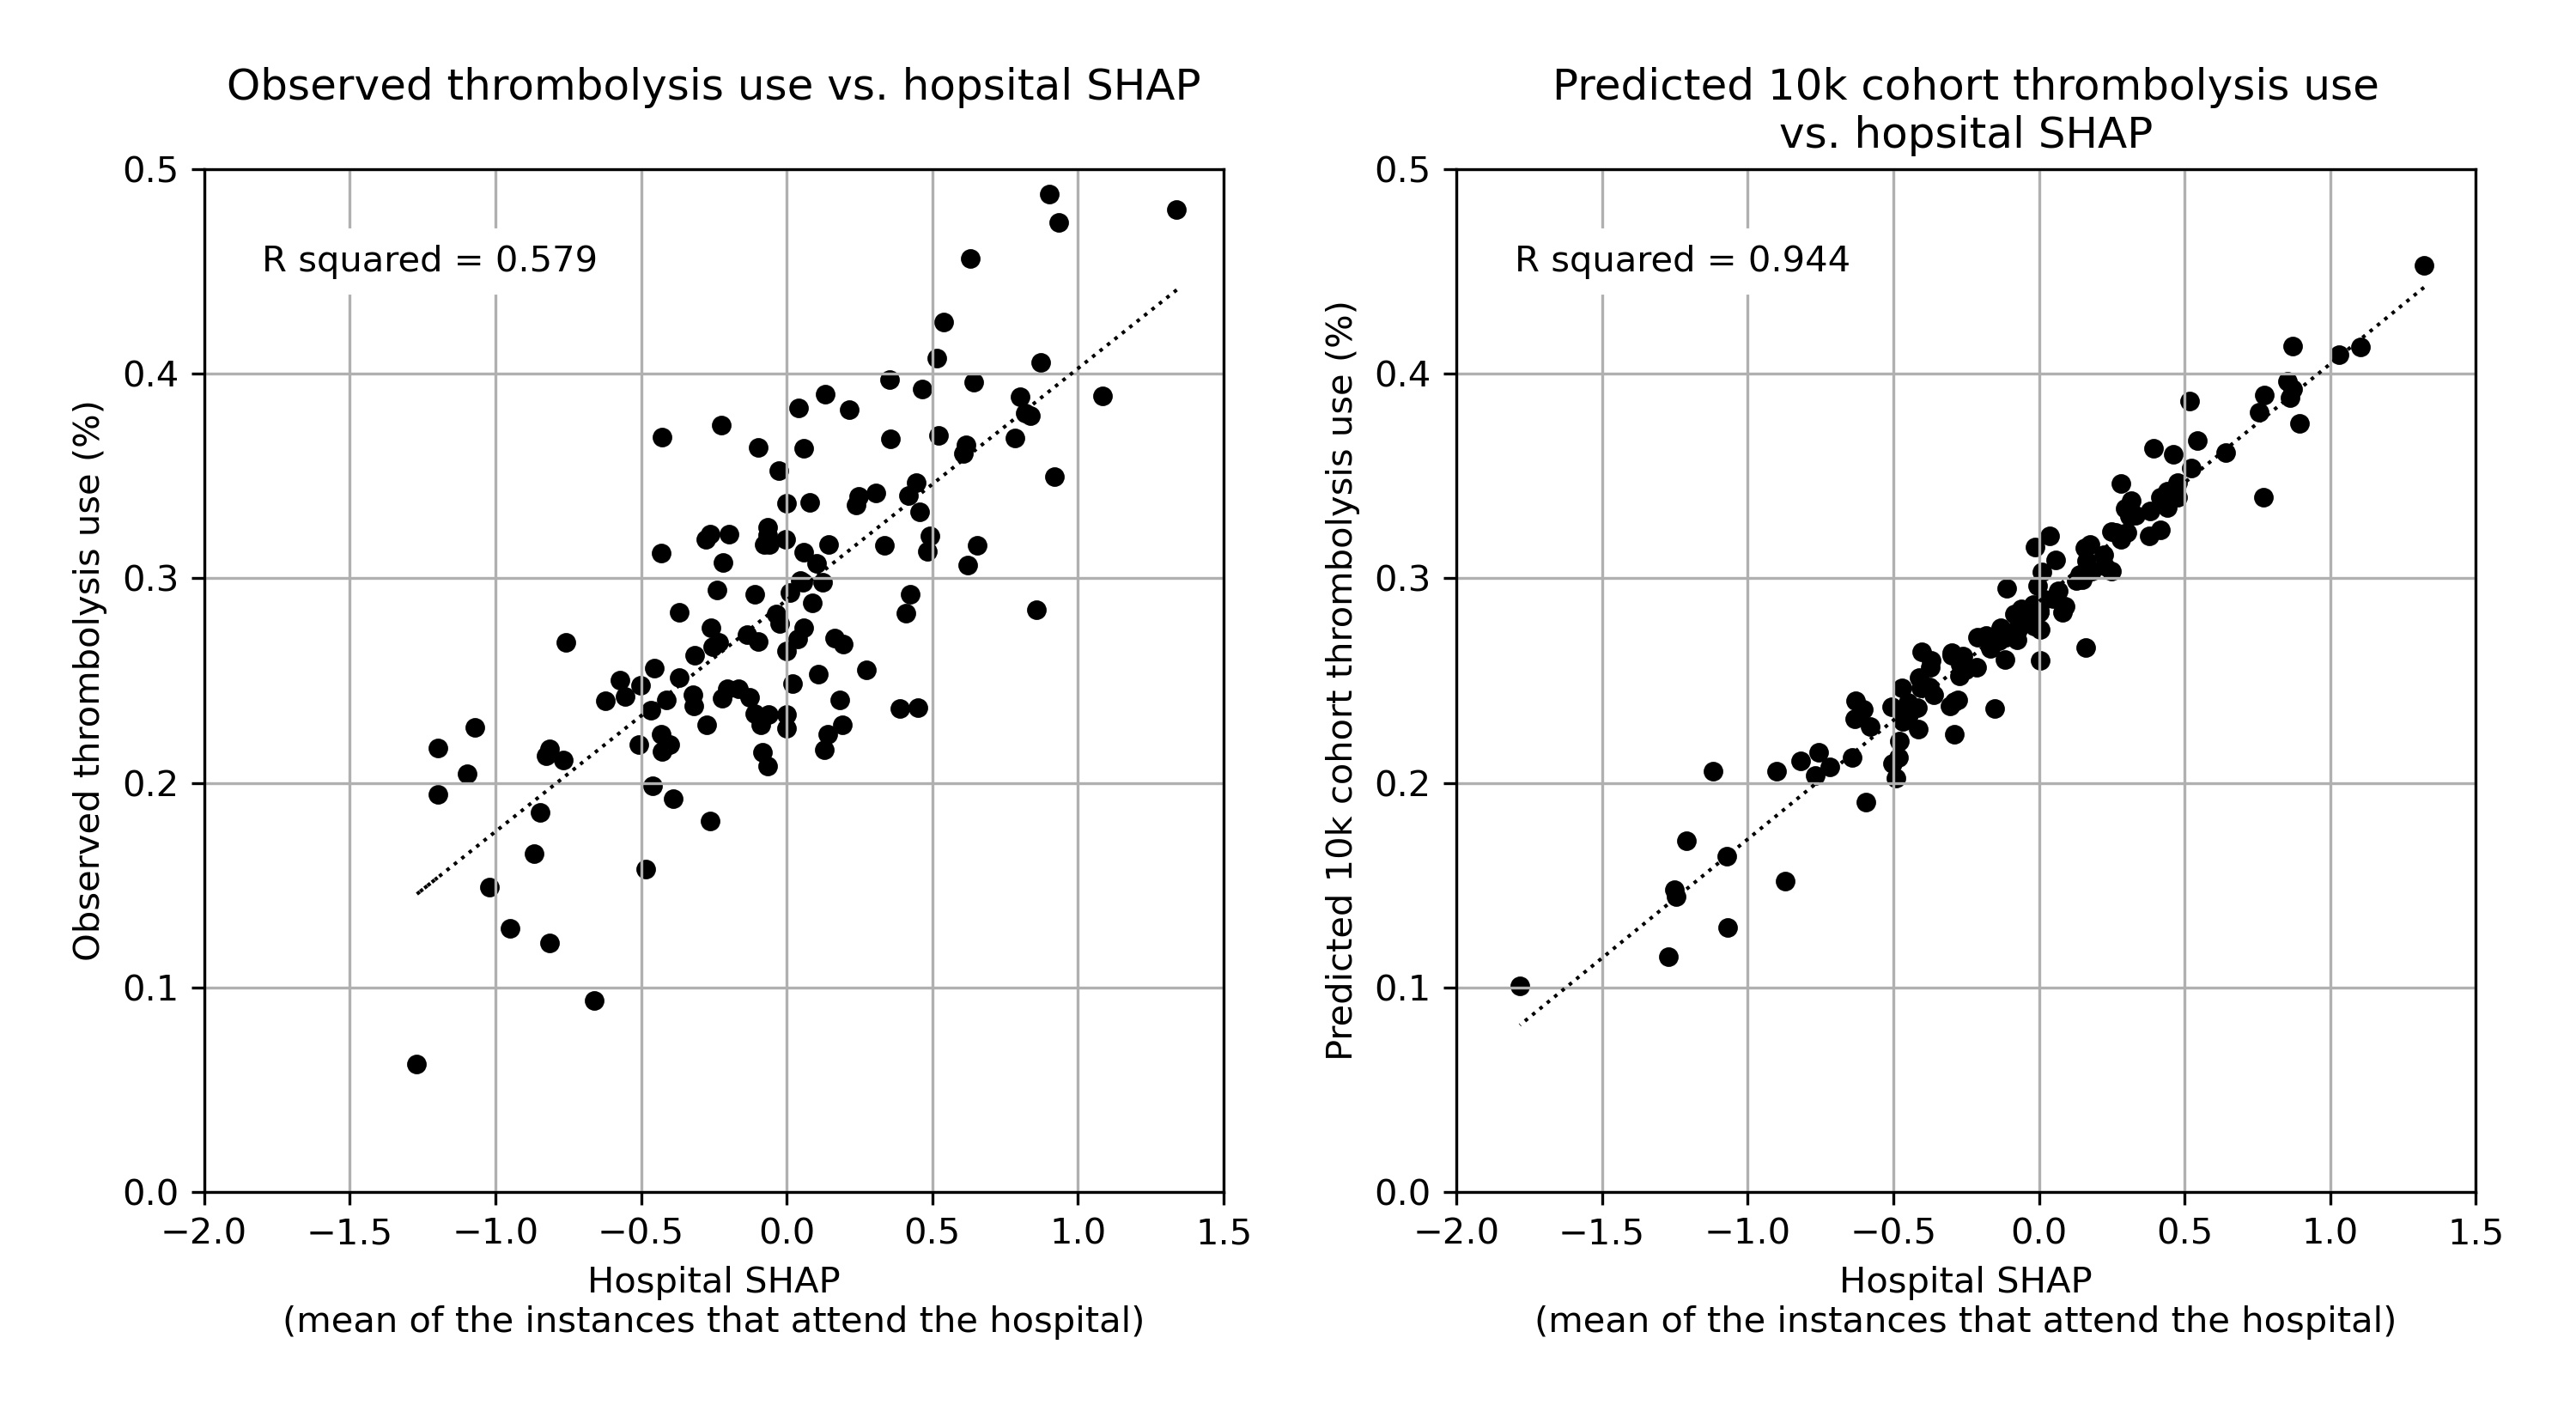
\includegraphics[width=1.0\textwidth]{./images/99_twin_correlation_scatter.jpg}
\end{center}
\end{frame}

%%%%%%%%%%%%%%%%%%%%%%%%%%%%%%%%%%%%%%%%%%%%%%%%%%%%%%%%%%%%%%%

\begin{frame}
\frametitle{SHAP main effects and interactions}


\end{frame}

%%%%%%%%%%%%%%%%%%%%%%%%%%%%%%%%%%%%%%%%%%%%%%%%%%%%%%%%%%%%%%%

\begin{frame}
\frametitle{How general effects may be modified by individual hospitals}

\begin{center}
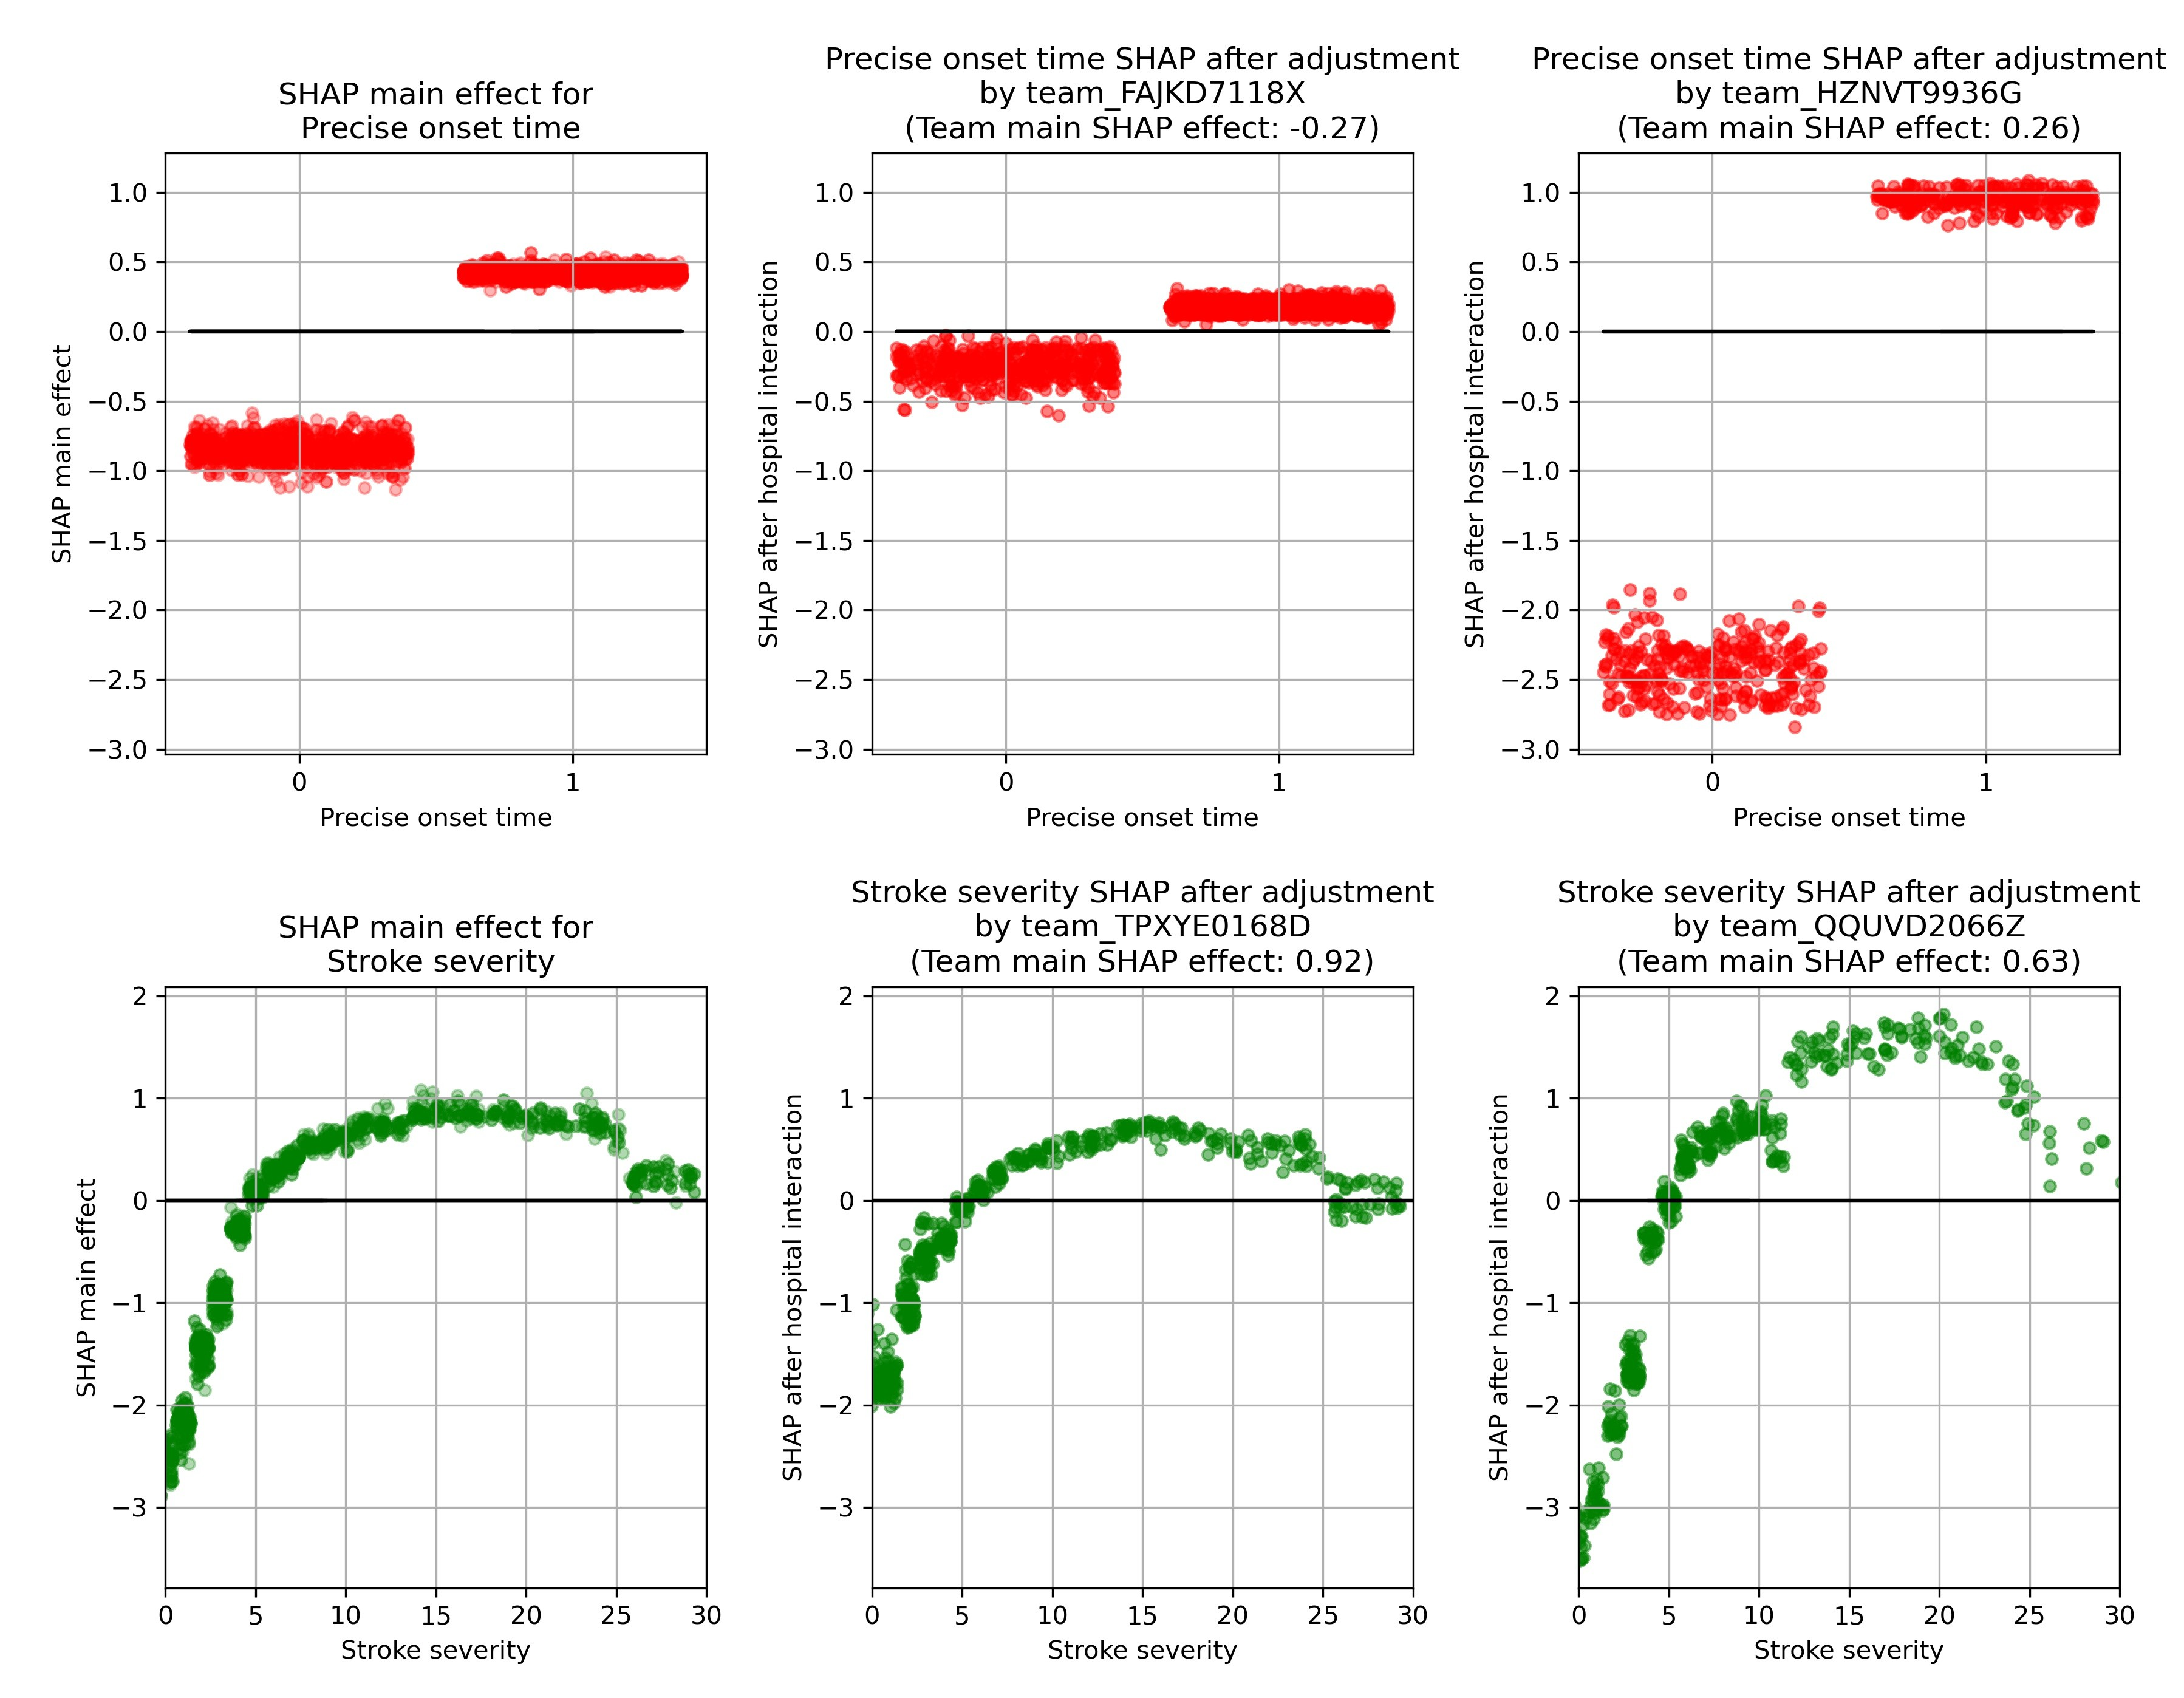
\includegraphics[width=0.88\textwidth]{./images/12aa_two_way_shap_adjustment.jpg}
\end{center}
\end{frame}

%%%%%%%%%%%%%%%%%%%%%%%%%%%%%%%%%%%%%%%%%%%%%%%%%%%%%%%%%%%%%%%

\begin{frame}
\frametitle{Thrombolysis in subgroups of patients (predicted use in a common 10k cohort at each team)}

\footnotesize The range of the predicted thrombolysis use across the 132 hospitals for subsets of the 10k patient cohort. The subsets of patients to the right of \emph{Ideal patients} all have the ideal patient characteristics with the specified changes

\begin{center}
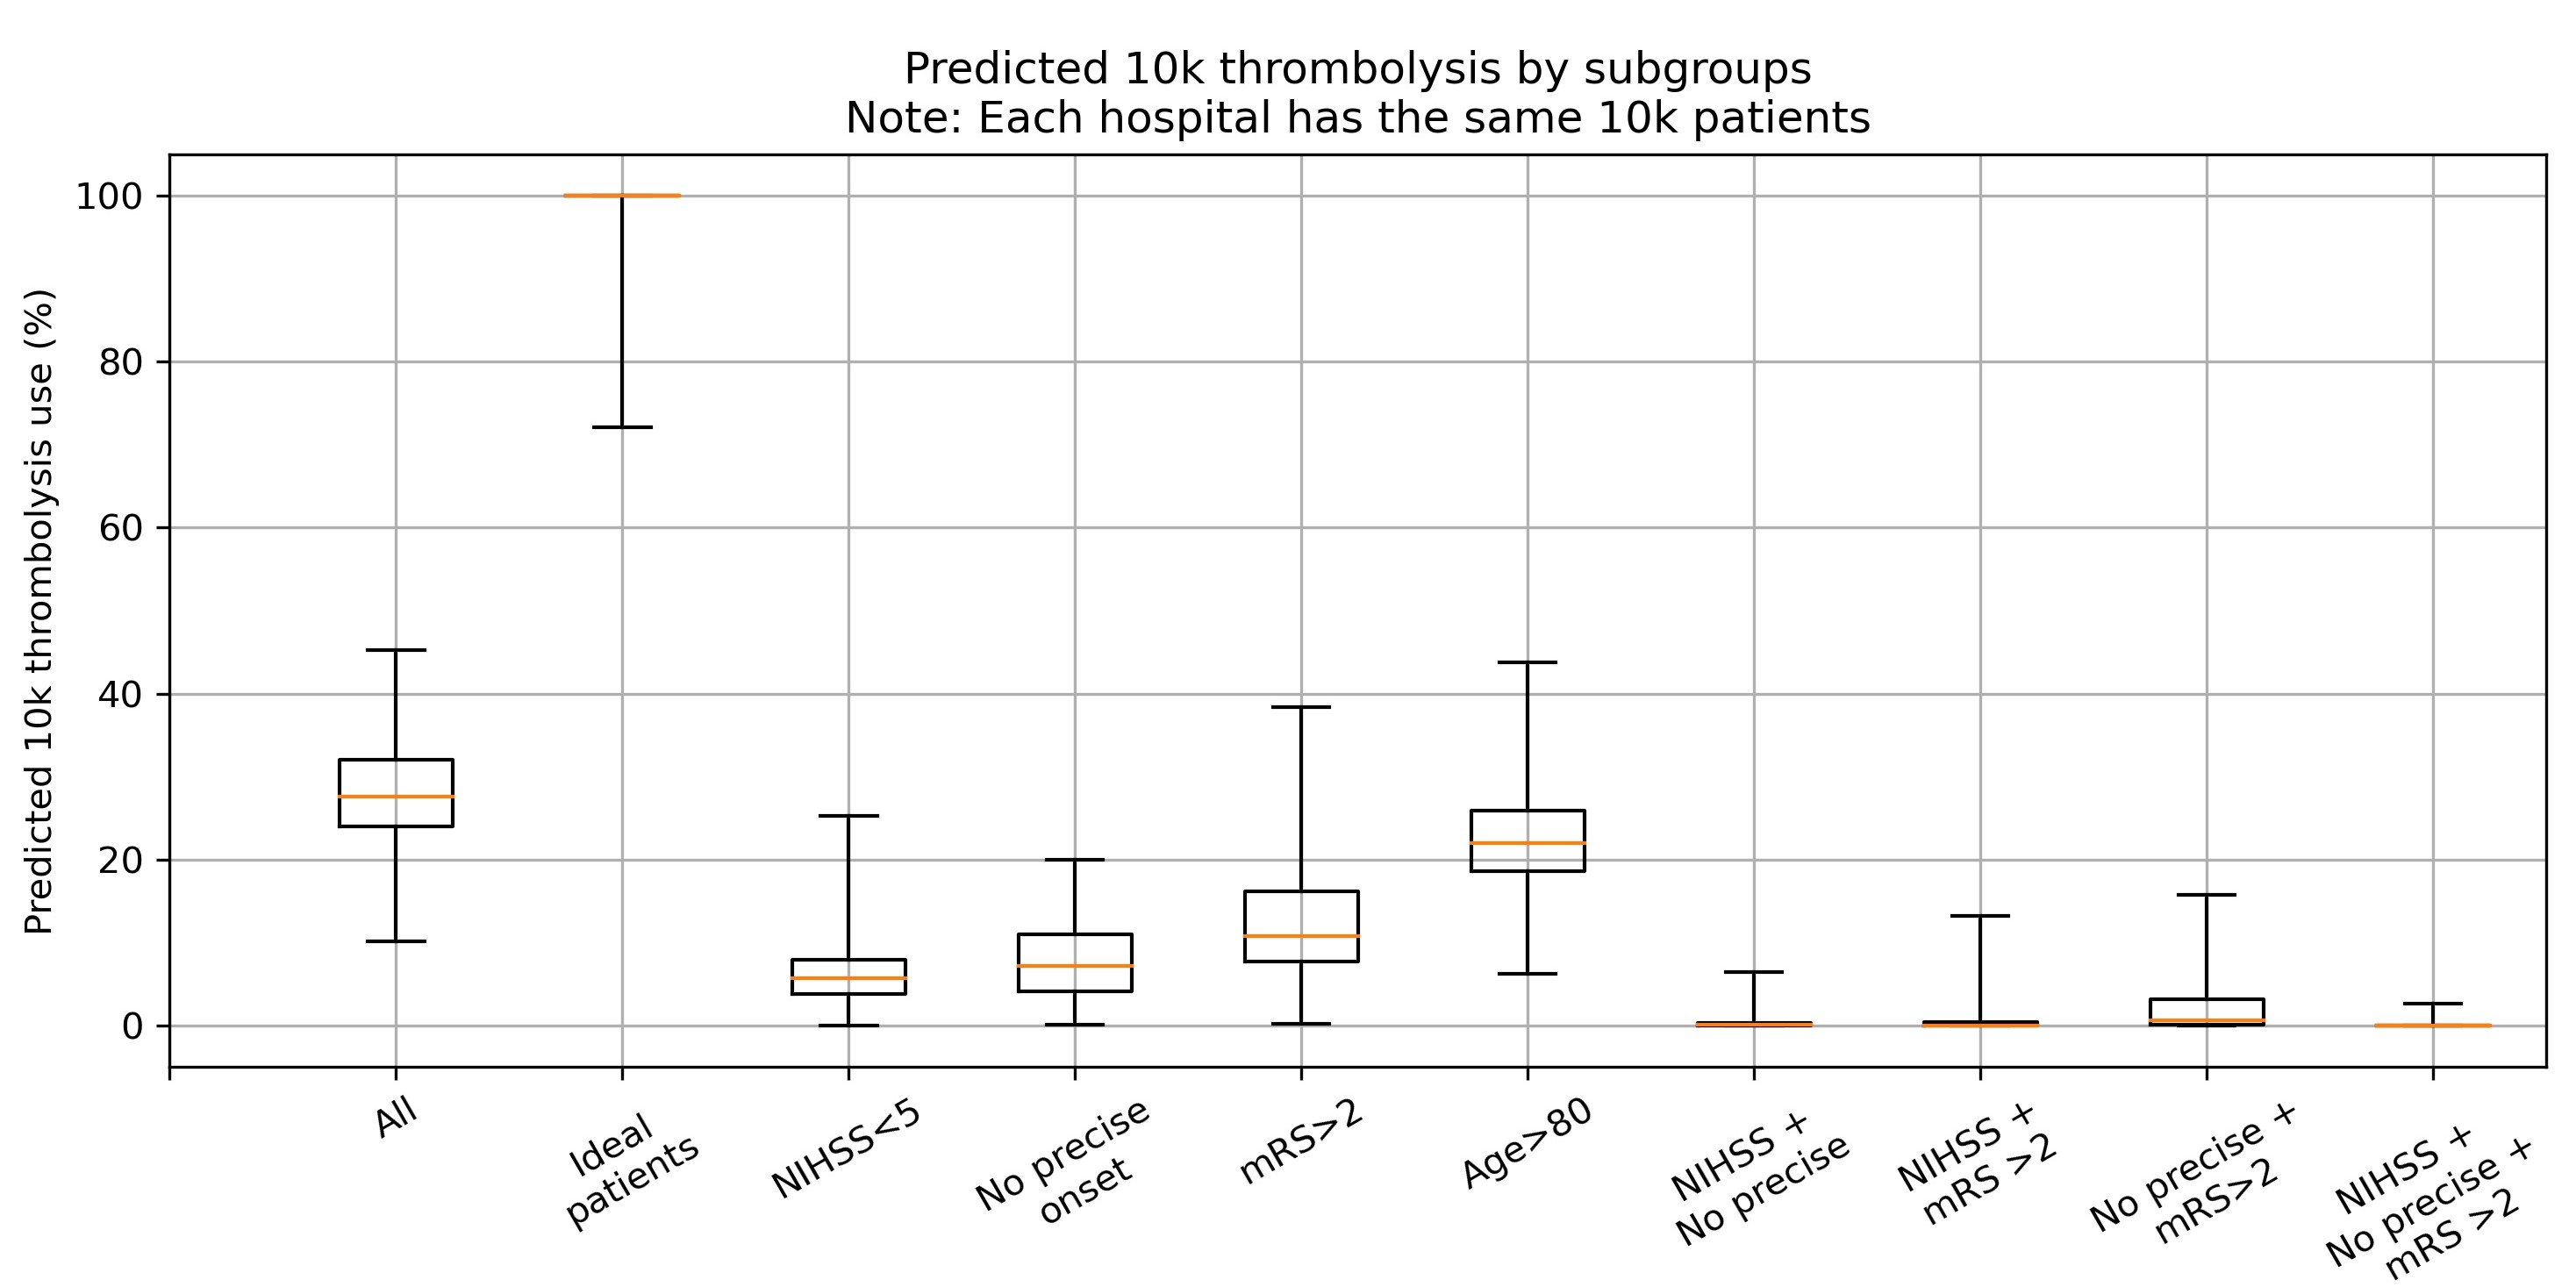
\includegraphics[width=0.83\textwidth]{./images/15c_modelled_subgroup_violin.jpg}
\end{center}

\scriptsize An \emph{ideal patient} has: Stroke severity NIHSS in range 10-25, Arrival-to-scan time \textless{} 20 minutes, Stroke type = infarction, Precise onset time = True, Prior disability level (mRS) = 0, No use of AF anticoagulants, Onset-to-arrival time \textless{} 90 minutes, Age \textless{80 years}, Onset during sleep = False
\end{frame}

%%%%%%%%%%%%%%%%%%%%%%%%%%%%%%%%%%%%%%%%%%%%%%%%%%%%%%%%%%%%%%%

\begin{frame}
\frametitle{Thrombolysis in subgroups of patients (observed use in each hospitals own patients)}

\footnotesize The range of the observed thrombolysis use across the 132 hospitals for subsets of the hospitals own patients. The subsets of patients to the right of \emph{Ideal patients} all have the ideal patient characteristics with the specified changes.

\begin{center}
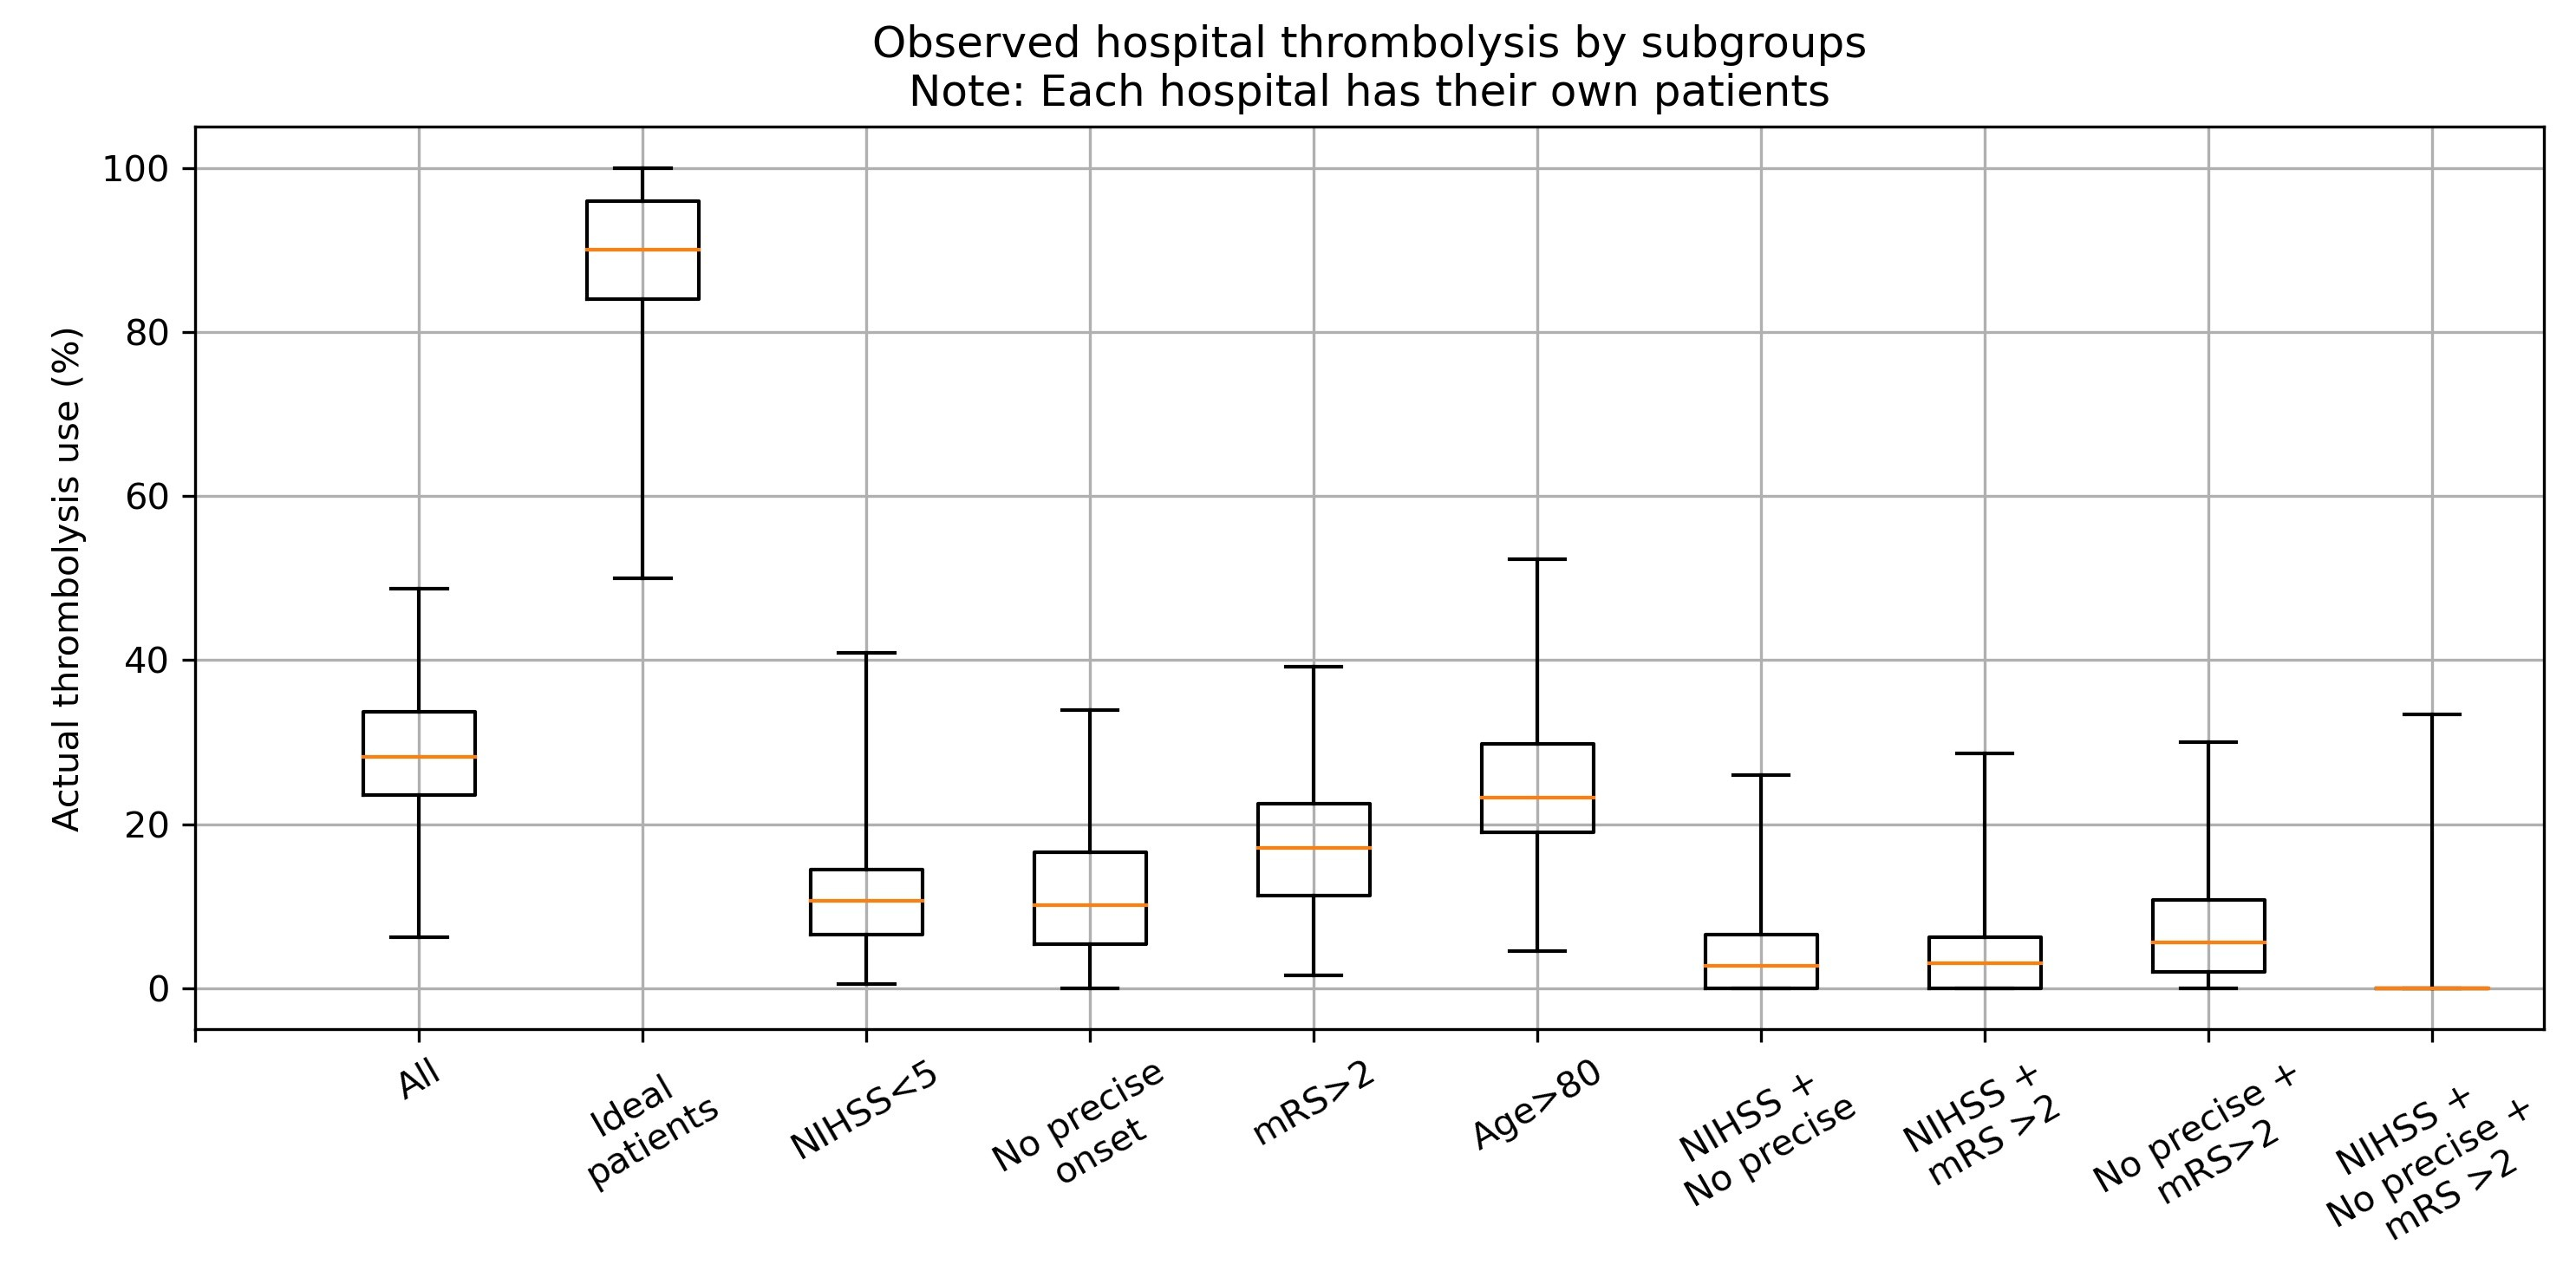
\includegraphics[width=0.83\textwidth]{./images/15b_actual_subgroup_violin.jpg}
\end{center}


\scriptsize An \emph{ideal patient} has: Stroke severity NIHSS in range 10-25, Arrival-to-scan time \textless{} 20 minutes, Stroke type = infarction, Precise onset time = True, Prior disability level (mRS) = 0, No use of AF anticoagulants, Onset-to-arrival time \textless{} 90 minutes, Age \textless{80 years}, Onset during sleep = False
\end{frame}

%%%%%%%%%%%%%%%%%%%%%%%%%%%%%%%%%%%%%%%%%%%%%%%%%%%%%%%%%%%%%%%

\begin{frame}
\frametitle{Thrombolysis in subgroups of patients (predicted use in a common 10k cohort at each hospital)}

    \begin{center}
    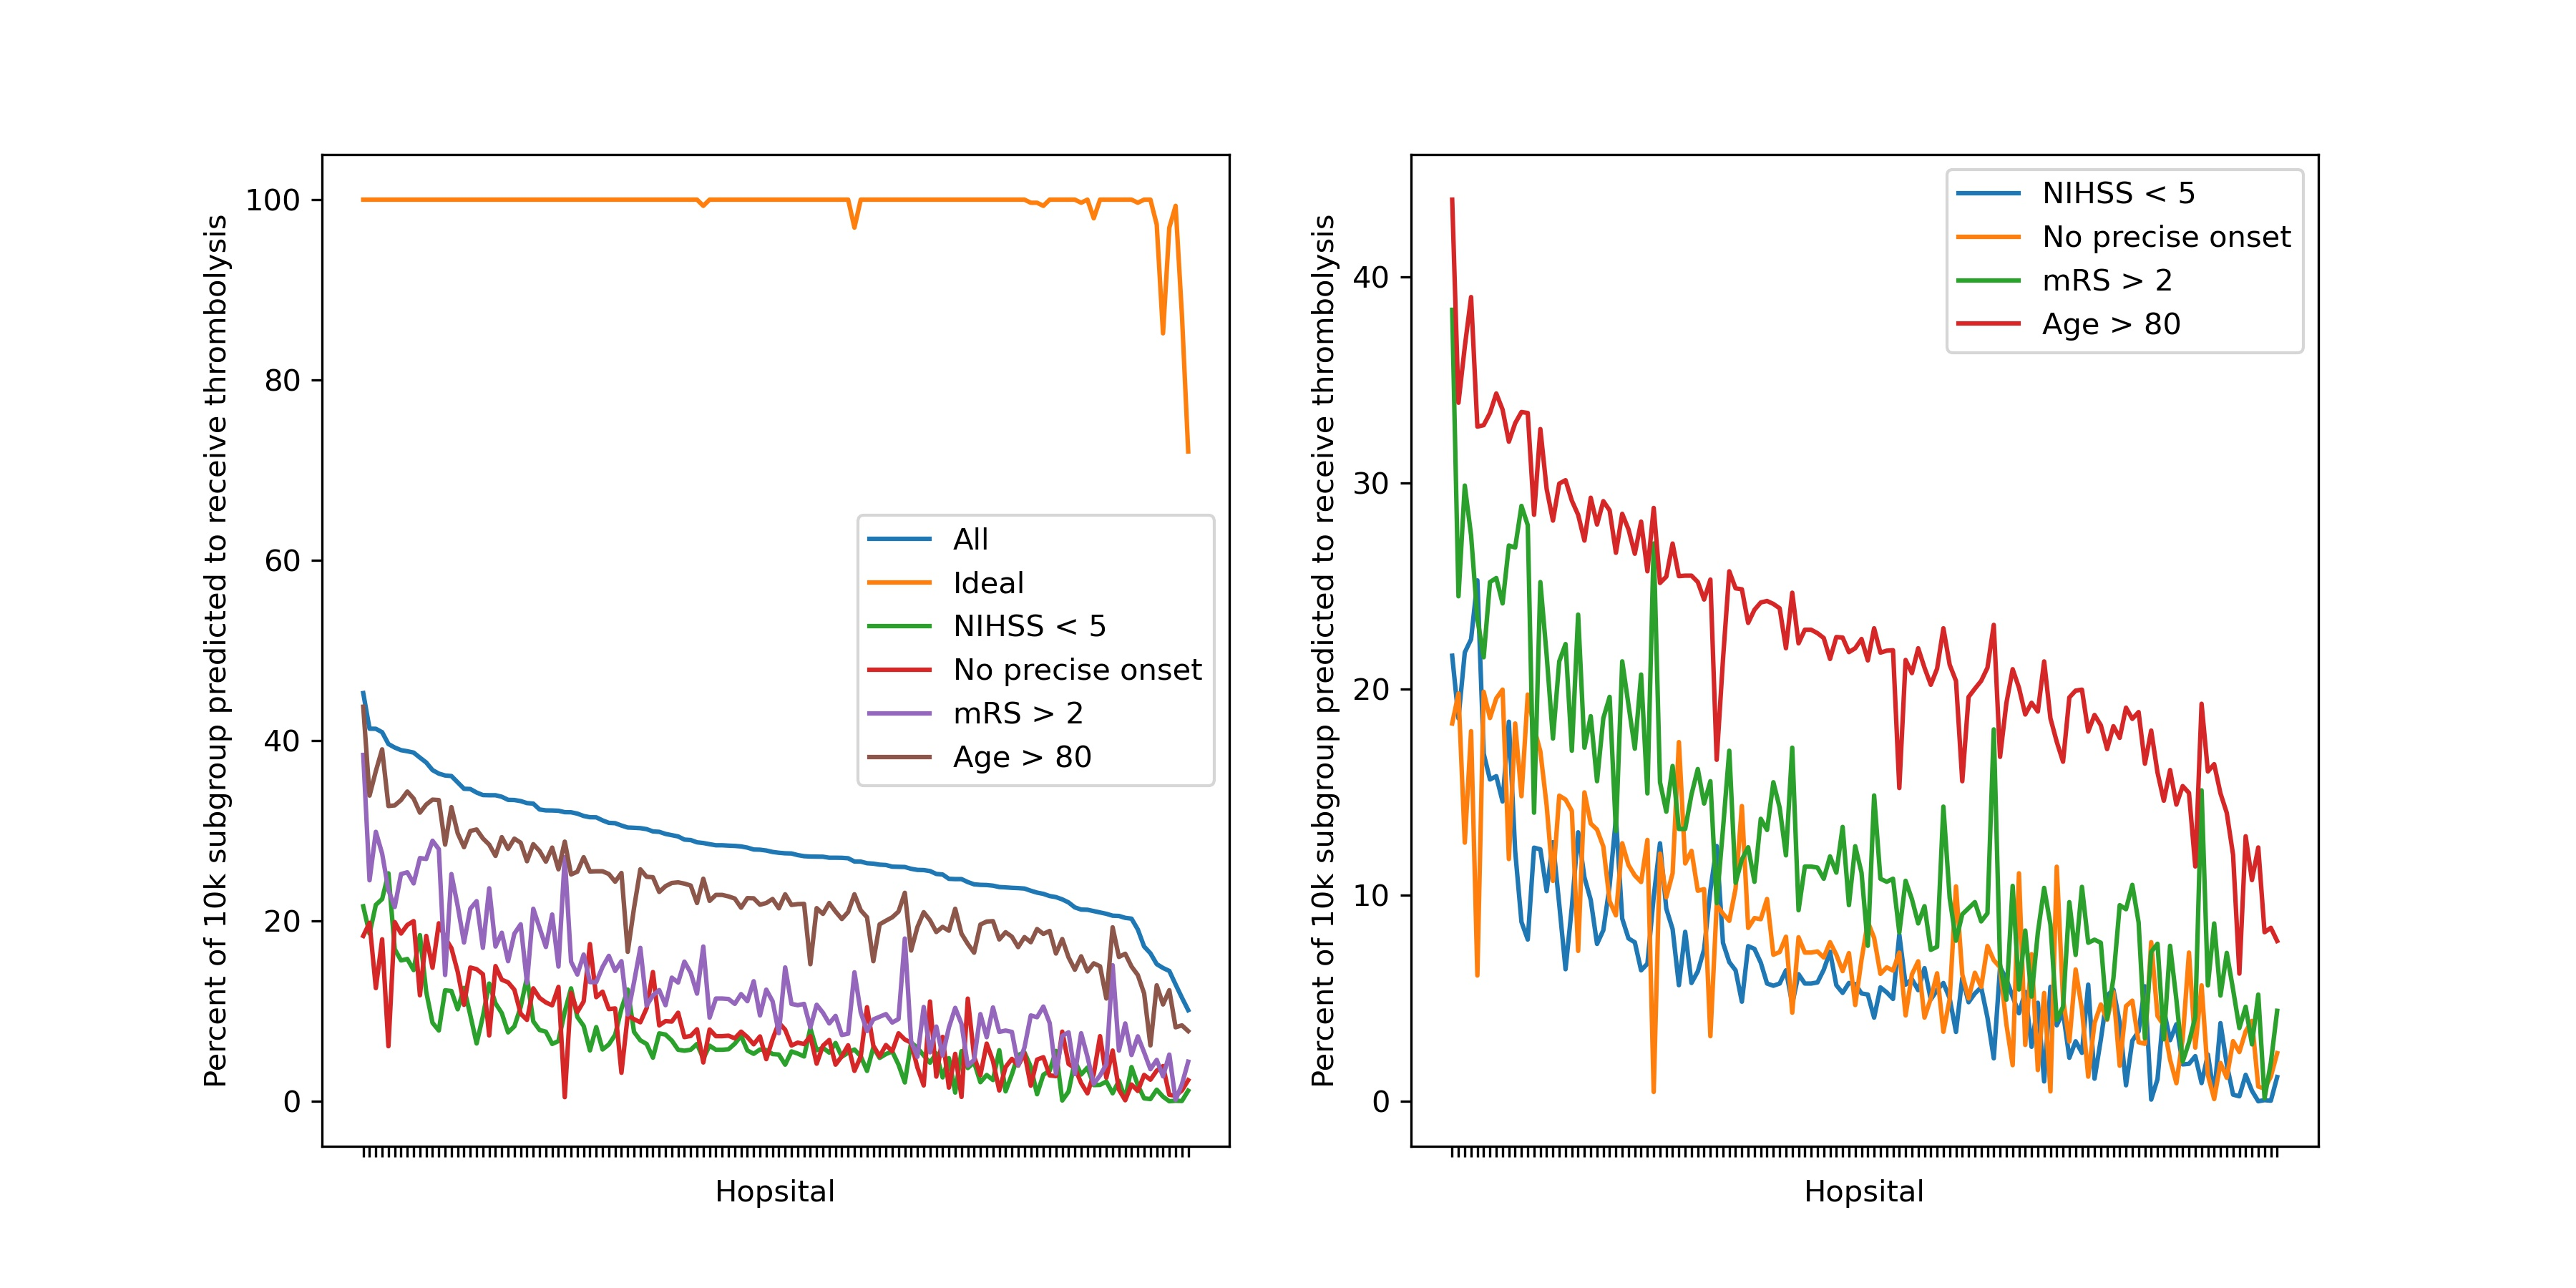
\includegraphics[width=0.90\textwidth]{./images/15_10k_subgroup.jpg}
    \end{center}

\footnotesize Hospitals with lower thrombolysis use were particularly less likely to give thrombolysis to patients with milder strokes, prior disability, or patients with imprecise onset time.
\newline
\newline
\footnotesize Note: Subgroups, other than \emph{ideal patients}, tend to track each other.  

\end{frame}



\begin{frame}
\frametitle{Thrombolysis in subgroups of patients (observed use in each hospitals own patients)}

    \begin{center}
    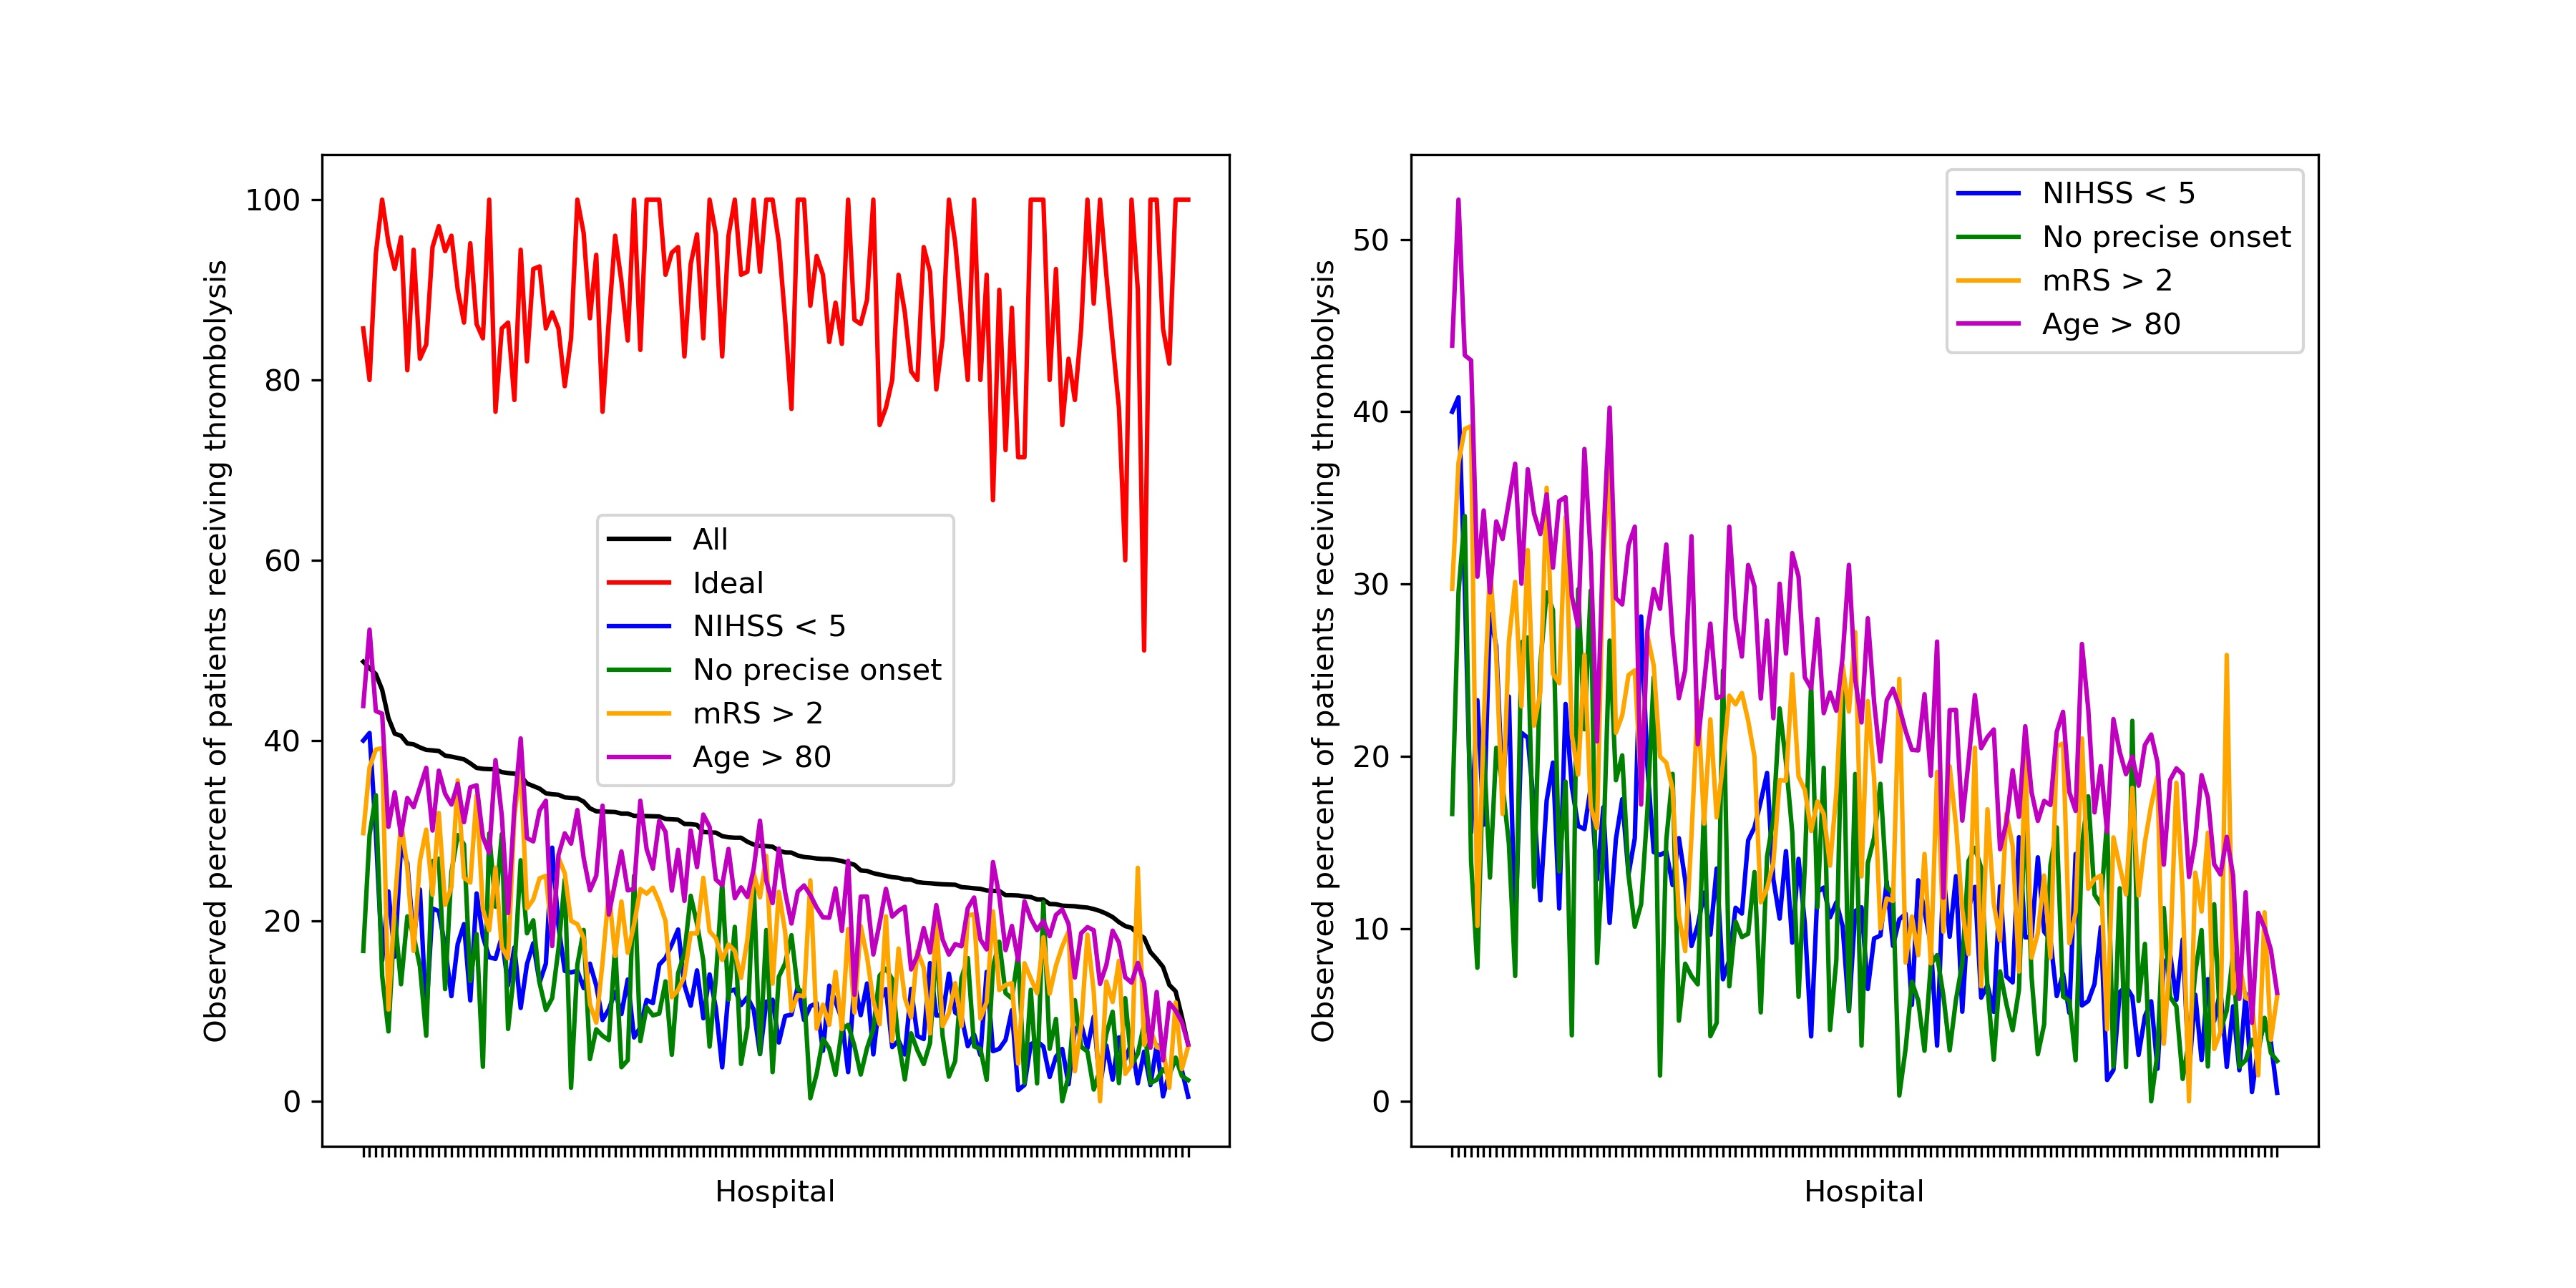
\includegraphics[width=0.9\textwidth]{./images/15a_actual_subgroup.jpg}
    \end{center}

\footnotesize Note: Subgroups, other than \emph{ideal patients}, tend to track each other, but with more noise than predicted thrombolysis use. 

\end{frame}

%%%%%%%%%%%%%%%%%%%%%%%%%%%%%%%%%%%%%%%%%%%%%%%%%%%%%%%%%%%%%%%


\begin{frame}
\frametitle{Investigating how hospitals differ in thrombolysis decision-making: Artifical patients}

\vspace{3mm}

\begin{columns}[t]
    \begin{column}{0.45\textwidth}
        Base patient:
        \begin{itemize}
            \footnotesize
            \item Onset to arrival = 80 mins
            \item Arrival to scan = 20 mins
            \item Infarction = Yes
            \item NIHSS = 15
            \item Prior disability level = 0
            \item Precise onset time = Yes
            \item Use of AF anticoagulents = No
        \end{itemize}
    \end{column}
    
    \begin{column}{0.5\textwidth}
    Proportion of hospitals predicted to give thrombolysis:
    \footnotesize
    \begin{itemize}
        \item Base patient: 99\%
    \end{itemize}
    Base patient with:
    \begin{itemize}
        \item NIHSS = 4: 73\%
        \item Pre-stroke mRS = 3: 86\%
        \item Estimated stroke onset time: 64\%
    \end{itemize}
    \end{column}

\end{columns}
\end{frame}


%%%%%%%%%%%%%%%%%%%%%%%%%%%%%%%%%%%%%%%%%%%%%%%%%%%%%%%%%%%%%%%

\begin{frame}
\frametitle{How would different teams respond to the same patient?}

    \begin{center}
    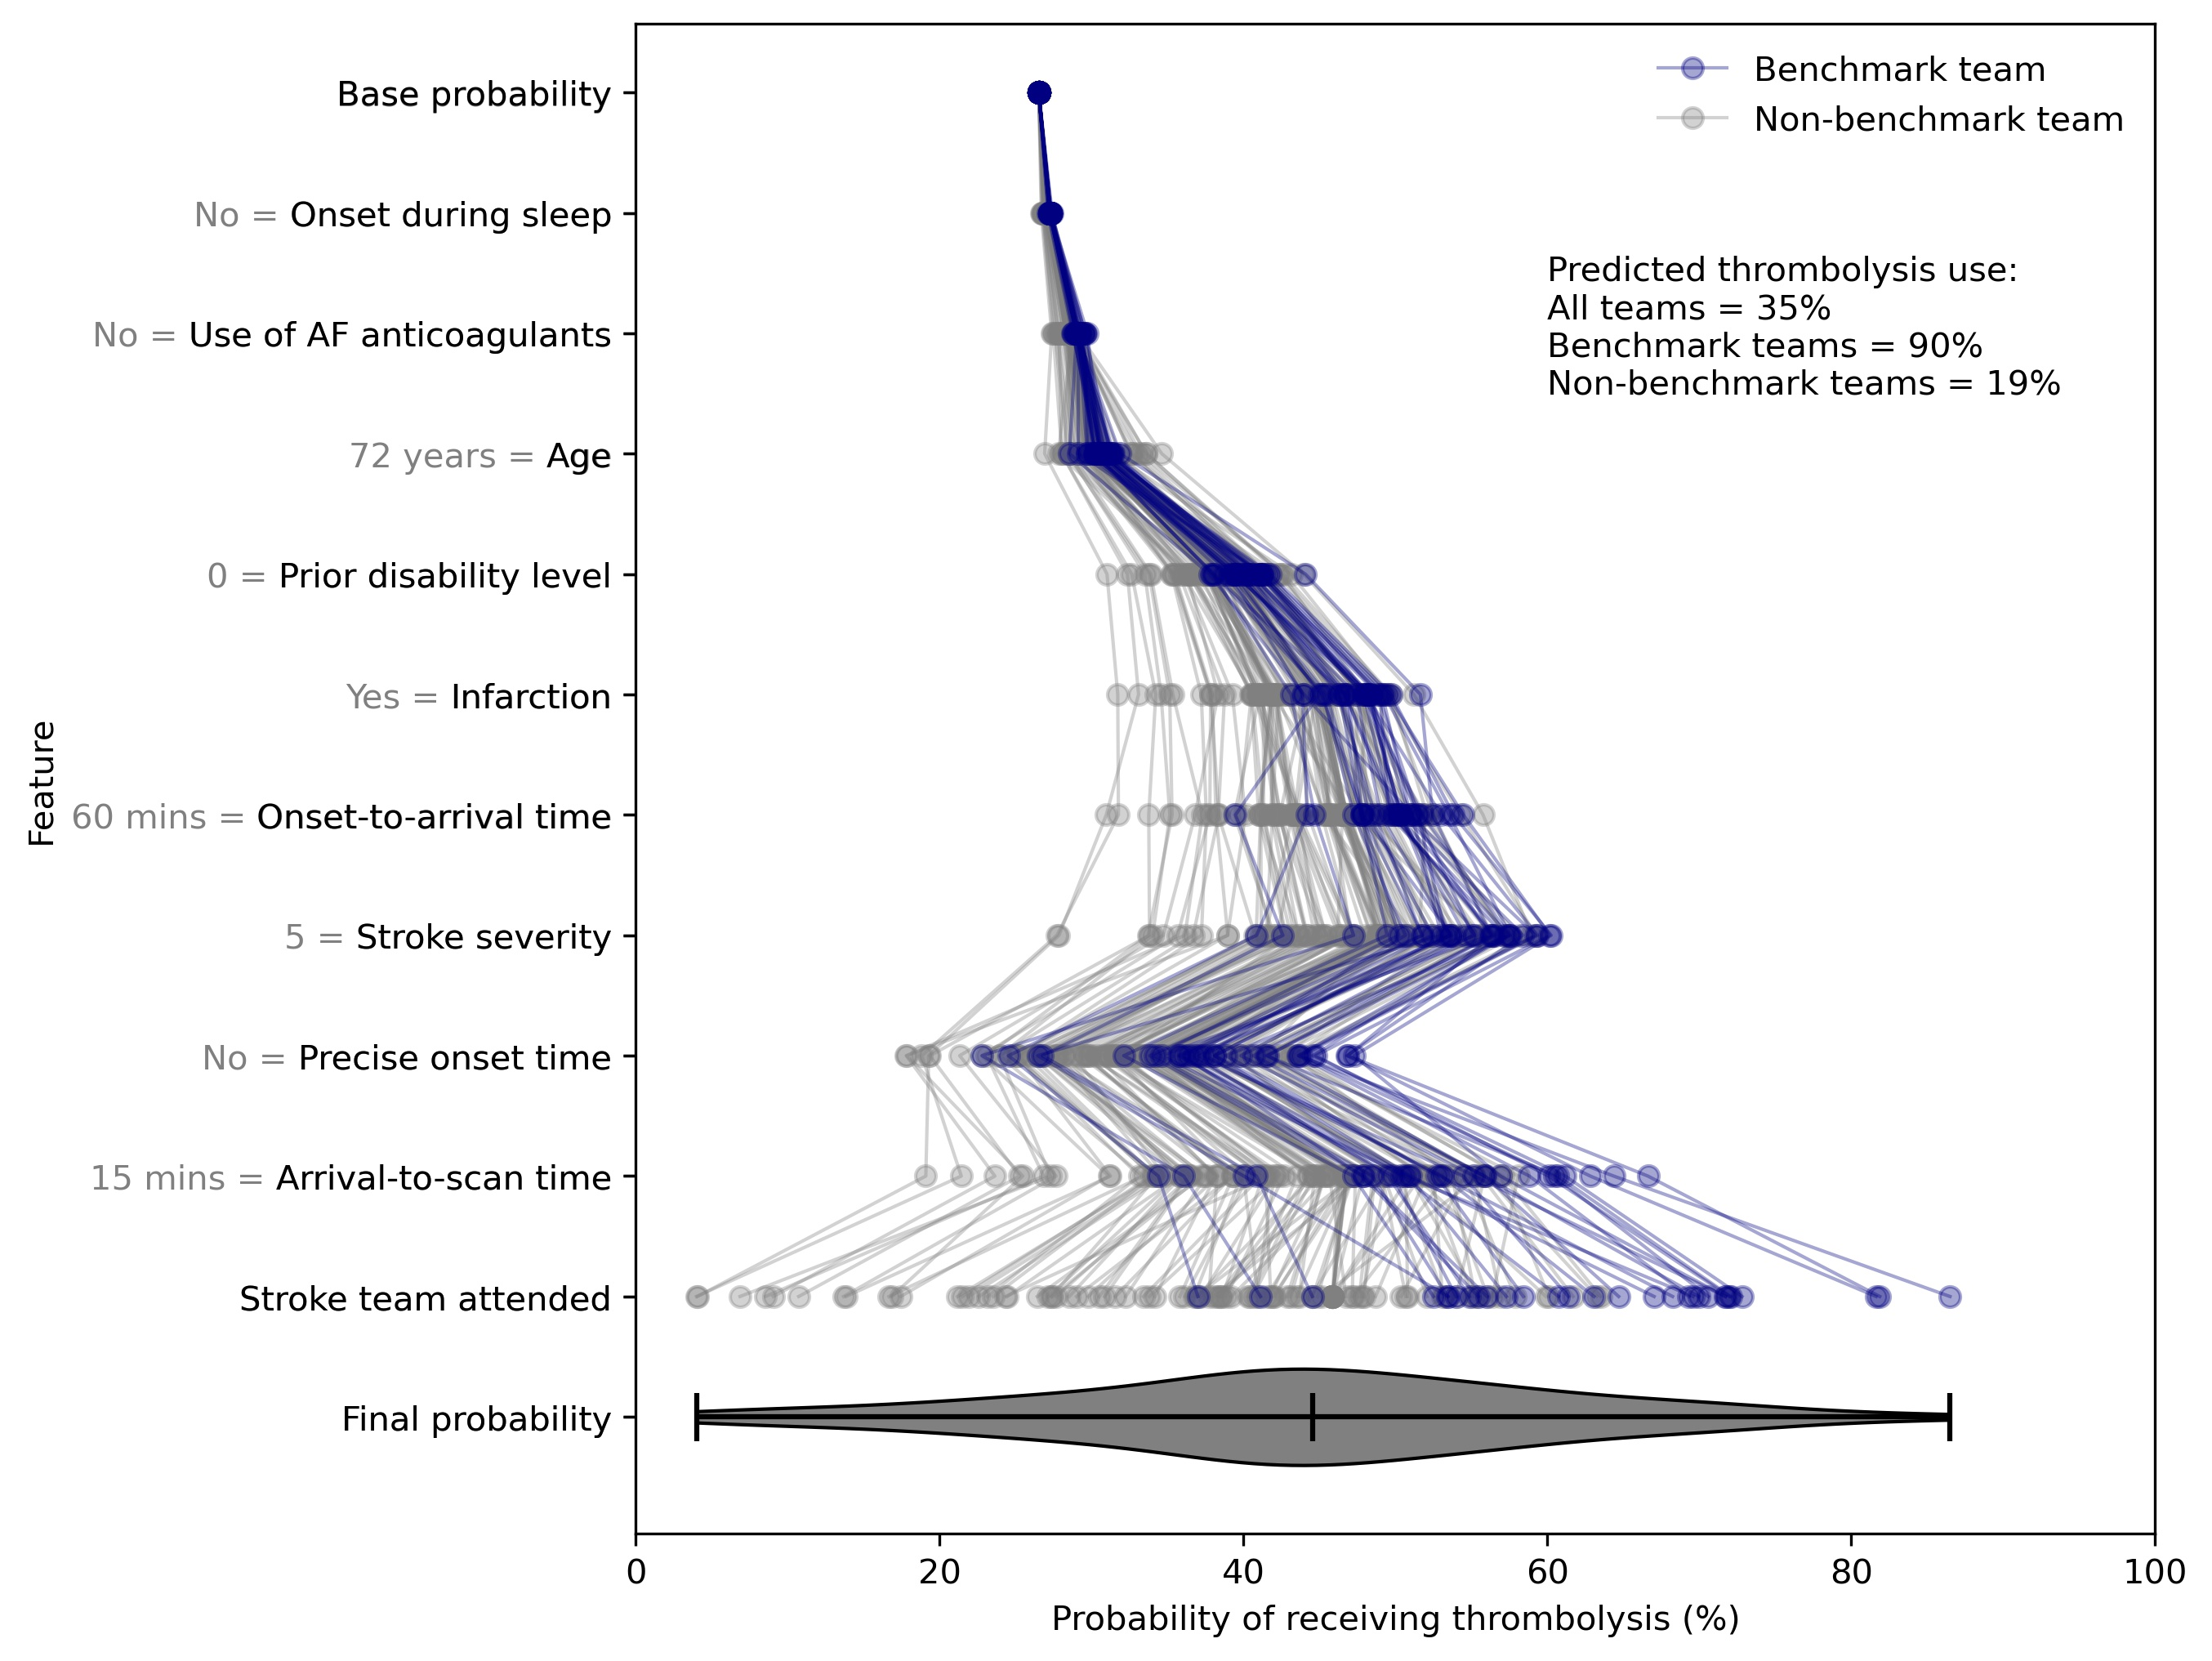
\includegraphics[width=0.7\textwidth]{./images/21_shap_waterfall_with_violin_contentious.jpg}
    \end{center}

\footnotesize The patient starts with the same base probability, then each hospital reacts differently when presented with each of the patients characteristics and nudges the probability to a different level.

\end{frame}


%%%%%%%%%%%%%%%%%%%%%%%%%%%%%%%%%%%%%%%%%%%%%%%%%%%%%%%%%%%%%%%

\begin{frame}
\frametitle{Summary}
\small

\begin{itemize}
    \item The XGBoost/SHAP model revealed that the odds of receiving thrombolysis:

    \begin{itemize}
        \item Reduced with increasing arrival-to-scan time.
        \item Varied 30 fold depending on stroke severity.
        \item Reduced with imprecisely known onset time.
        \item Fell with increasing pre-stroke disability.
        \item Varied 15 fold between hospitals. 
    \end{itemize}

\item The hospital identification (hospital SHAP value) explained 58\% of the variance in between-hospital thrombolysis use. 

\item Compared with hospitals with higher thrombolysis use, hospitals with lower use were particularly less likely to give thrombolysis to patients with milder strokes, prior disability, or patients with imprecise onset time.
\end{itemize}

\end{frame}

%%%%%%%%%%%%%%%%%%%%%%%%%%%%%%%%%%%%%%%%%%%%%%%%%%%%%%%%%%%%%%%


\end{document}




